\documentclass[12pt]{report}
\usepackage{color}
\usepackage{amsmath,mathtools}
\usepackage{amsthm}
\newtheorem{myLemma}{Lemma}[section]
\newtheorem{thm}{Theorem}[section]
\usepackage{chngcntr}
\counterwithin{figure}{section}
\counterwithin{table}{section}
\usepackage{amssymb}
\usepackage{graphicx}
\usepackage{multirow}
\usepackage{csvsimple,longtable}%For importing csv files
\usepackage{listings,framed,systeme}
\usepackage{float}

\usepackage[inline]{enumitem} 

\usepackage{hyperref}
\hypersetup{
    colorlinks=true,
    linkcolor=blue,
    filecolor=blue,      
    urlcolor=cyan,
    citecolor=red,
    linktocpage=true
}
\usepackage[utf8]{inputenc}
%\usepackage[english]{babel}
\inputencoding{utf8}



\title{Machine Learning and Feature Selection Analysis on Dynamic Connectivity Signatures in Neural Networks Engaged for Emotion Regulation}

\author{Emily Paul}

\begin{document}
	
	\maketitle
	\tableofcontents
	
	\chapter{Introduction}
	Major Depressive Disorder (MDD) is a mental disorder characterized by persistent low mood, loss of interest, and a reduction in the ability to regulate emotion. Its prevalence, especially in younger demographics, makes it a growing concern \cite{nimh_2019}. Unfortunately, many of the criteria for diagnosis listed in the Diagnostic and Statistical Manual of Mental Disorders, Fourth Edition, such as feelings of guilt, difficulty concentrating, and suicidal ideation, are highly subjective and difficult to quantify. This lack of conclusive biomarkers makes this disorder difficult to diagnose consistently \cite{lemelin1994depression}. This study aims to discover some quantitative features that can aid in the classification of potential patients. Creating a machine learning model that can quantitatively and reliably distinguish between patient and non-patient data would greatly improve the diagnosis process. Over the course of this project, some preliminary machine learning and feature selection analysis was conducted on a range of subject data including functional Magnetic Resonance Imaging (fMRI) time series encapsulating changing levels of activity in different brain regions during emotional regulation.
	
	All scripts referred to in the report can be found in the \\ MachineLearning$\_$NeuroscienceProject repository at  \url{https://github.com/VeraLiconaResearchGroup/MachineLearning_NeuroscienceProject.git}.
	
	\chapter{Background Information}
		\section{Neuroscience Data Collection}
		Dr. Mike Stevens and his team at the Olin Neuropsychiatry Research Center collected data from 129 adolescents ranging in age from 12 to 18 years. 105 of the subjects had no history of mental disorders and were classified as healthy. The remaining 24 subjects were in remission from MDD. For each subject, the team recorded phenotypic data by administering tests such as the Beck Depression Inventory, the Early Adolescent Temperament Questionnaire, and the Multidimensional Anxiety Scale for Children; the full list is included in the MachineLearning$\_$NeuroscienceProject repository. The researchers also collected data from 4 Functional Magnetic Resonance Imaging (fMRI) scans of the subject's brain. Where MRIs have been used to visualize the anatomical structure of the brain, fMRIs measure changes in cerebral bloodflow, and thus produced data in time series encapsulating the changing levels of metabolic activity in different brain regions. Over the course of each scanning period, the subject was shown a series of images, each designed to evoke an emotional response. During two of the scans, subjects were asked to heighten their emotional response to the presented stimuli, and during the other two scans, they were asked to repress the response to the best of their ability. Thus, the team produced 4 time series per subject, two each for increased and decreased emotional response.
	
		\section{Data Processing}
		Dr. Paola Vera-Licona and her team at the Center for Quantitative Medicine at UCONN Health created a pipeline to extract a dynamic conectivity signature (dynamic signature) from each time series of fMRI data. They represented each time series as a probabilistic boolean network (PBN): a collection of the possible boolean networks that could solve for the fMRI time series. They then represented each PBN as an adjacency matrix, $ [a_{ij}] $, \\
		where $ a_{ij} = \dfrac{\text{number of times node i is input to node j}}{\text{total number of inputs to node j}} $.\\
		 As shown in Fig. \ref{networkgraph}, these matrices can be visualized as graphs in which nodes are brain regions and edges are interactions between them. An edge exists between node $i$ and node $j$ if $a_{ij} \neq 0$. In the graph in Fig. \ref{networkgraph}, both node size and node color are mapped to betweenness centrality, which is a measure of the degree to which a node falls in the shortest path between any two other nodes. Large, purple nodes have high betweenness centrality, and thus act as hubs in the network, while small, yellow nodes have low betweenness centrality. Similarly, edge density is mapped to edge betweenness; heavier edges have higher edge betweenness. The networks were visualized this way to make them easier to interpret.
		
		\begin{figure}[H]
			\centering
			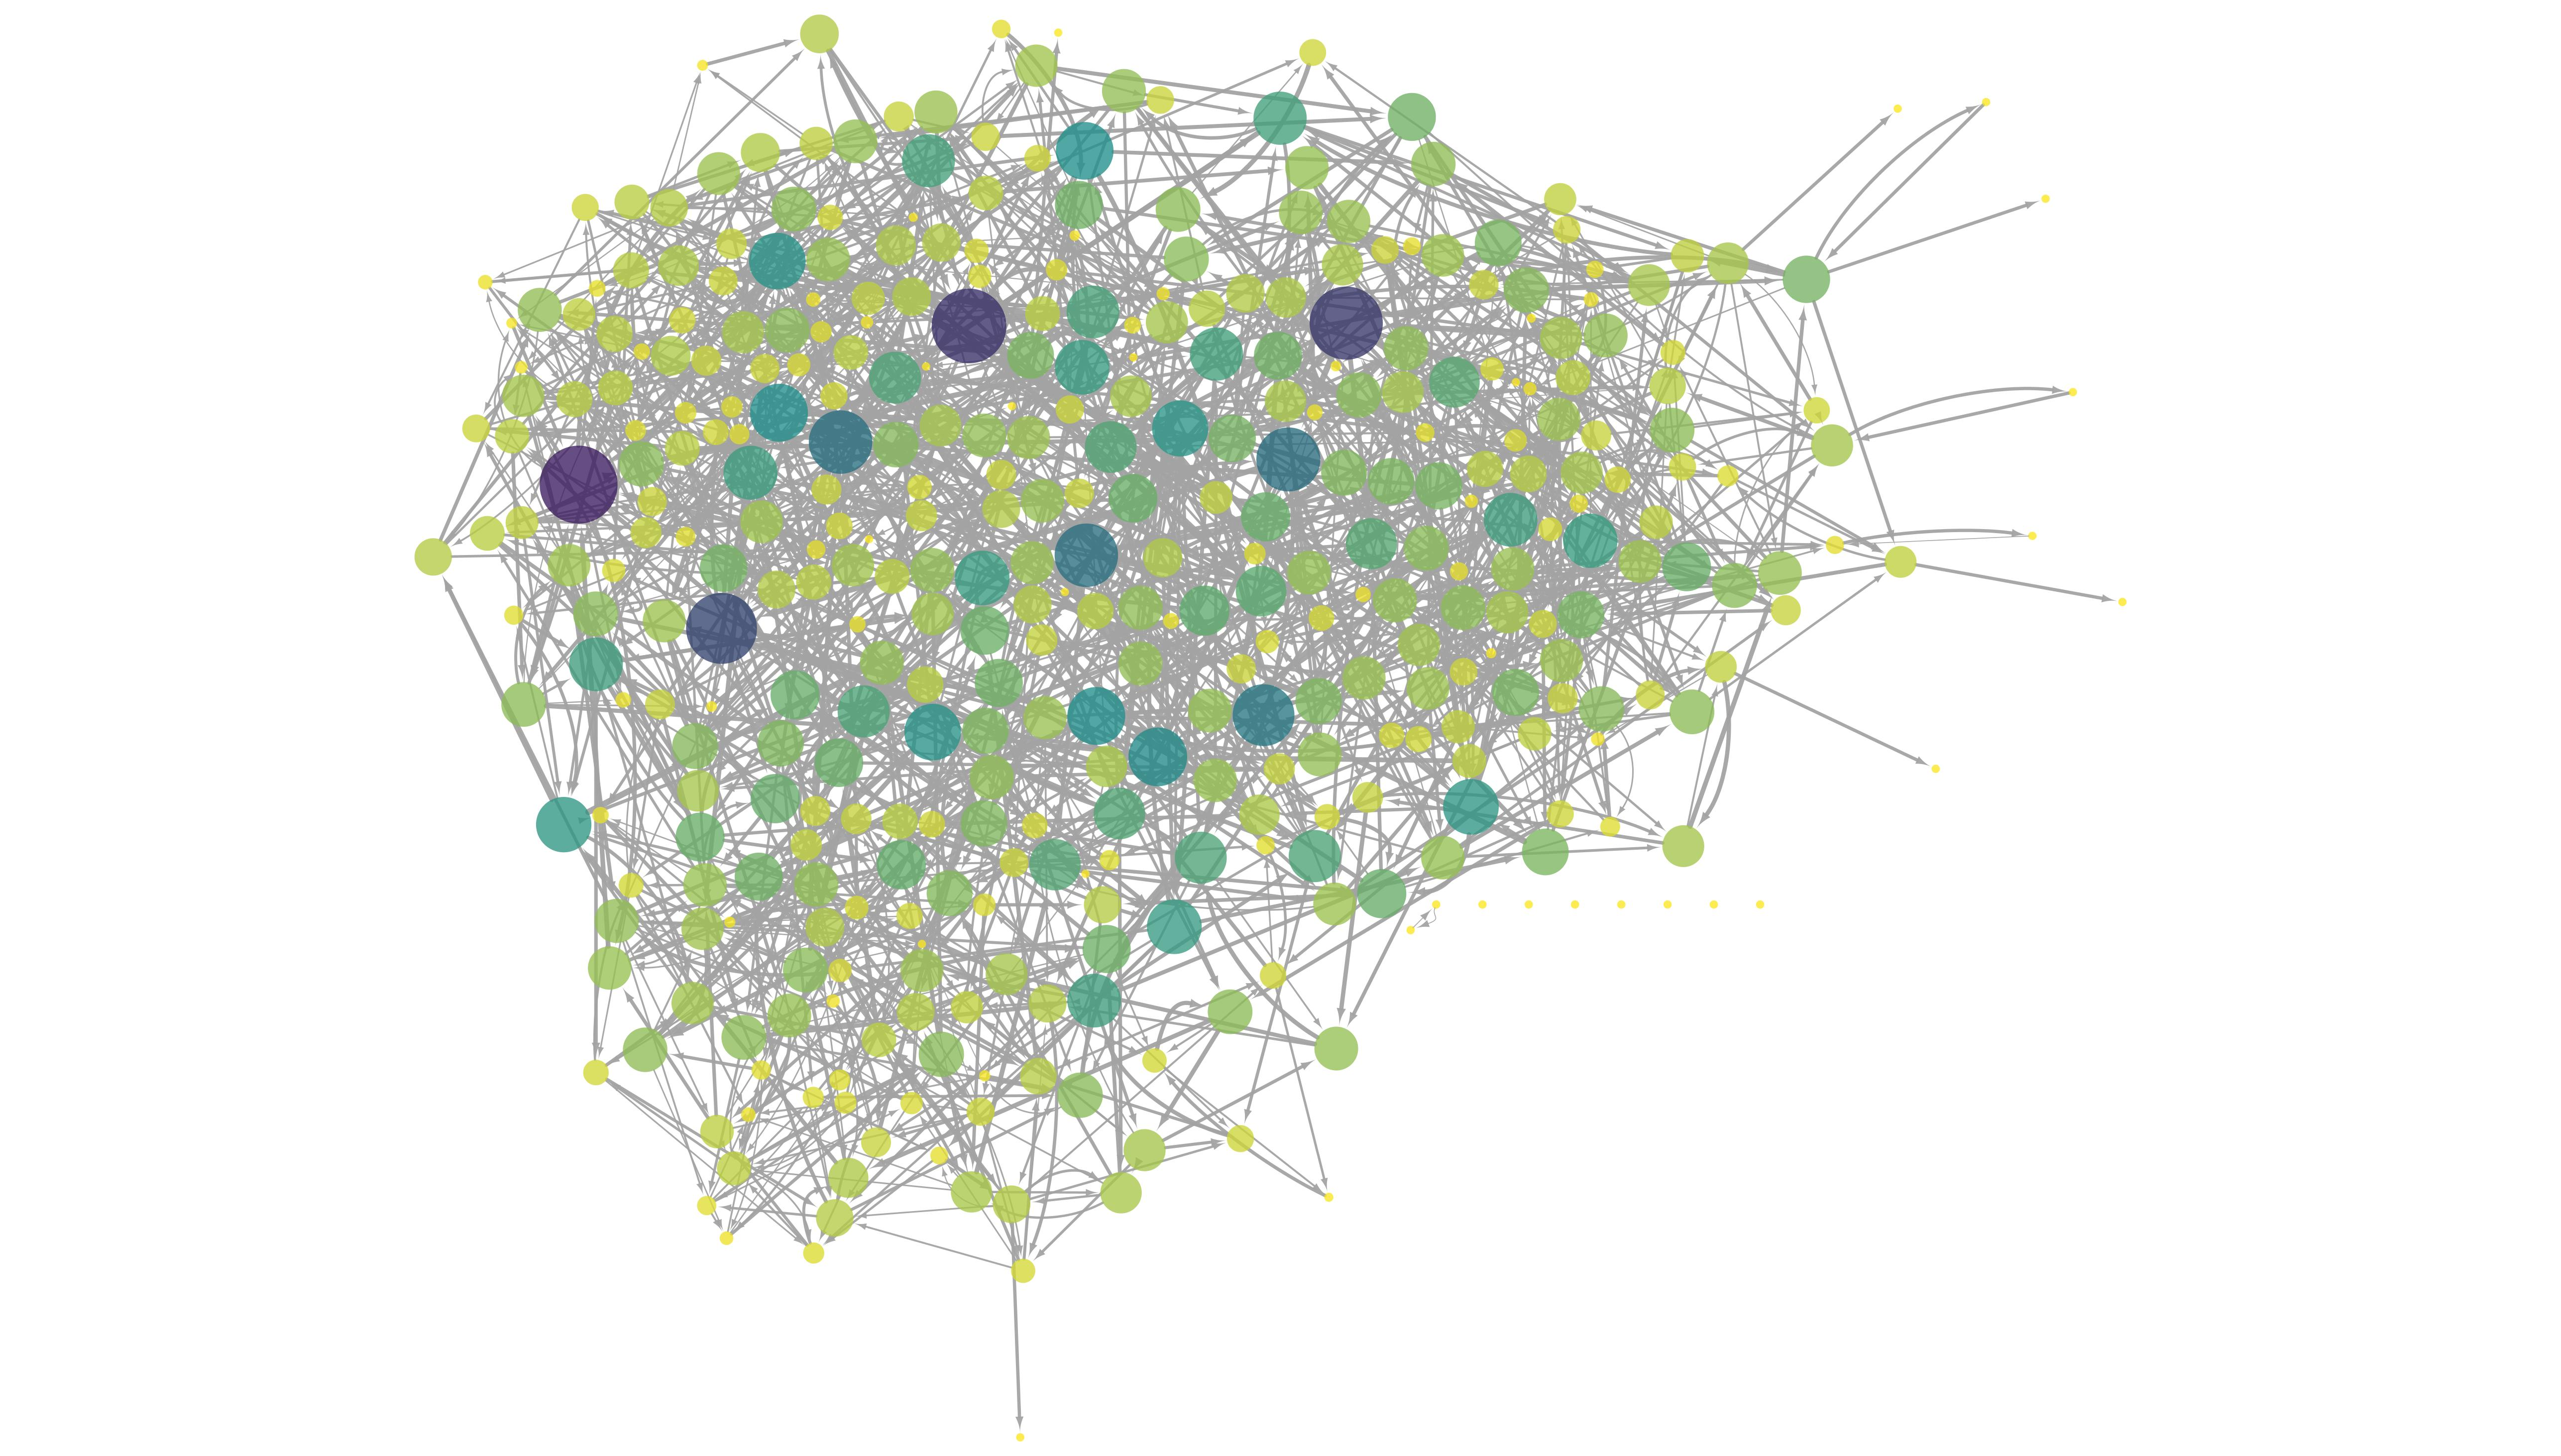
\includegraphics[scale=0.075]{Images/S0197BMS2INCLRcompletecorr_DynSig_k4.jpeg}
			\caption{Dynamic signature graph}
			\label{networkgraph}
		\end{figure}
		
	\chapter{Data Mining}
		\section{Conserved Components in Dynamic Signatures}
		After checking for intersections among the dynamic signatures (see the script creating$\_$intersection$\_$networks.R), it was observed that there were several subgraphs which were conserved across over 75$\%$ of the dynamic signatures. Of these, the connected components shown in Fig. \ref{amygdalahippocampuscomponent} were of particular interest. They involve the same brain regions and display identical connectivity, in the right and left hemispheres. These components illustrate activity in the amygdala-hippocampal complex, which has been established to be a driver of emotion regulation. It controls the formation of episodic memories in response to stimuli and modulates cognitive appraisal \cite{phelps2004human}. Studies have uncovered some potential associations between amygdala \cite{Hamilton2008} and hippocampus \cite{Anand2017} core volume and MDD.

			\begin{figure}[H]
				\centering
			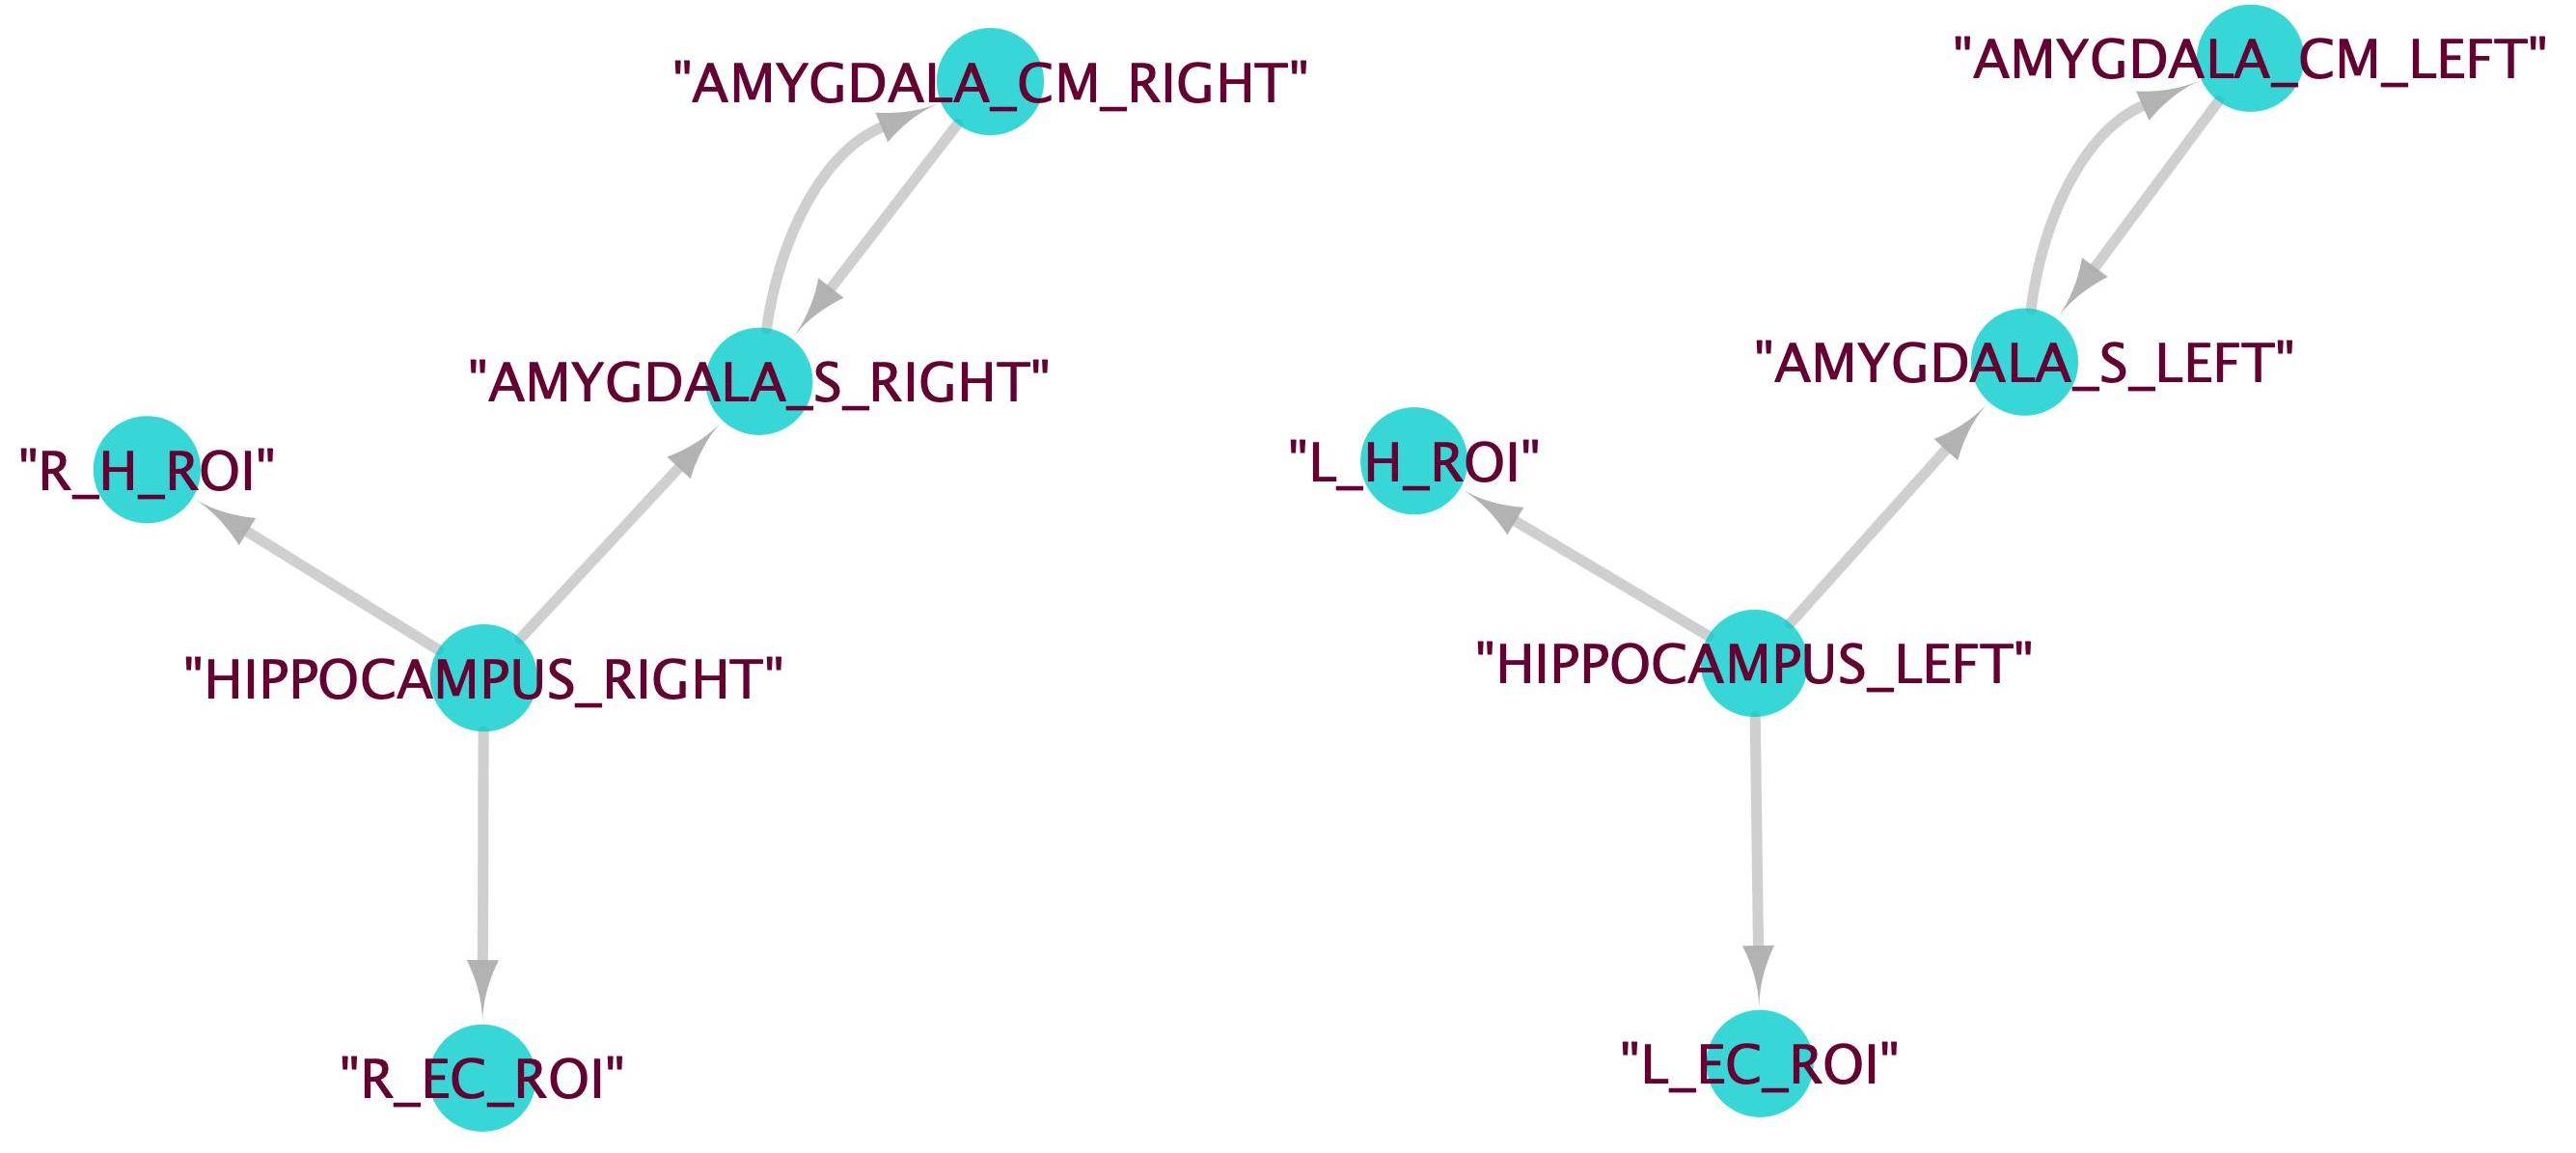
\includegraphics[scale=0.1]{Images/conserved_amygdala_hippocampal_complex.jpeg}
			\caption{Conserved amygdala-hippocampal complex}
			\label{amygdalahippocampuscomponent}
			\end{figure}
		
		\section{Features Generated for Dynamic Signatures}
			\subsection{Network Features}
			Network features were gathered using the iGraph package in R. All of the datasets used in the analysis can be constructed by running the scripts in the  MachineLearning$\_$NeuroscienceProject repository, starting with the construction of iGraph objects in the script creating$\_$iGraph$\_$objects.R.
				\subsubsection{General Network Characteristics}
				16 network characteristics were calculated for each dynamic signature. The list of characteristics can be found in the script general$\_$network$\_$features.R. The INCgraphstats dataset contains the characteristics calculated for both increased emotional response dynamic signatures per subject, and thereby has 32 features. The DECgraphstats dataset contains the characteristics calculated for both decreased emotional response dynamic signatures per subject.
			
				\subsubsection{Motif Occurrences}
				Two subgraphs were constructed for each dynamic signature based on the location of the hippocampus region (left or right); each subgraph consisted of one of the hippocampus regions and all of the nodes of first and second order connectivity to it. For each subgraph, the number of occurrences for each of 16 different motifs (each composed of 3 vertices) was calculated; see the script triad$\_$occurrences$\_$hippocampus$\_$subgraphs.R.
			
			\subsection{Phenotypic Data}
			Dr. Stevens and his team produced a set of 531 phenotypic characteristics per subject. Unfortunately, only 13 of those were complete; the remainder contained missing values for various subjects. Instead of introducing bias and potentially skewing results by introducing false data points, only the 13 complete variables were used in the analysis. The list of the complete variables can be retrieved from the script clinical$\_$data$\_$processing.R.
		
			\subsection{Data Collation}		
			The data was collated into a dataframe wherein each subject was a row and each feature was a column. All columns containing only zeros were removed before applying dimensionality reduction and machine learning techniques, leaving 203 features per subject; see the script subject$\_$data$\_$analysis.R. These features will subsequently be referred to as the subject data.
		
	\chapter{Dimensionality Reduction and Machine Learning}
		\section{Dimensionality Reduction}
		Principal component analysis (PCA) is a dimensionality reduction technique that produces a list of principal components which are linear combinations of the original variables. It is used to visualize high dimensional datasets in 2 or 3 dimensions by capturing as much variance as possible within the first 2 or 3 principal components \cite{james2013introduction}. The biplot for the PCA conducted on the subject data is shown in Fig. \ref{subjectdatapcabiplot}, and the scree plot is given in Fig. \ref{subjectdatapcascreeplot}. They were computed using the prcomp() function in R on the scaled and centered subject data and visualized using Dr. Jason Cory Brunson's ordr package for the R tidyverse; see the script subject$\_$data$\_$analysis.R.
		
		\begin{figure}[H]
			\centering
			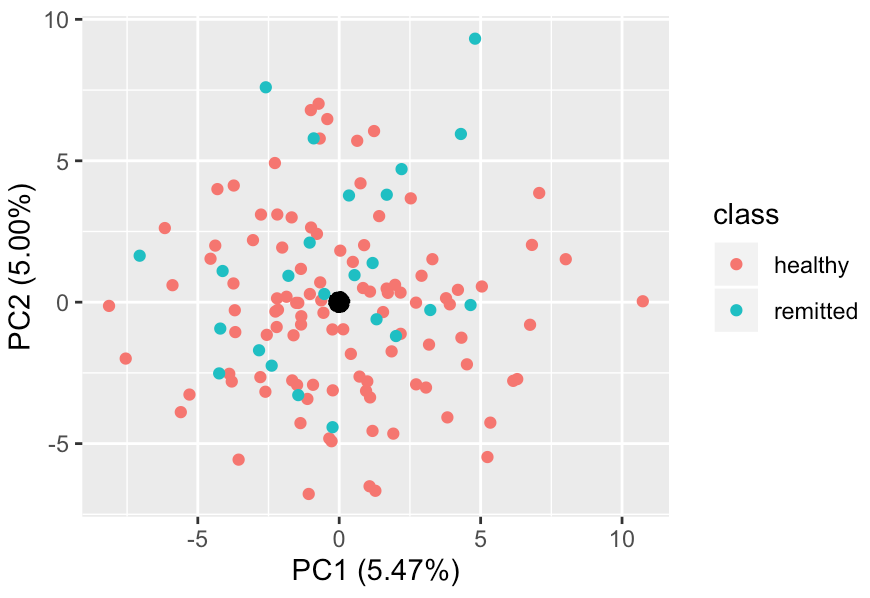
\includegraphics[scale=0.8]{Images/subjectdata_biplot.png}
			\caption{PCA biplot}
			\label{subjectdatapcabiplot}
		\end{figure}
	
		\begin{figure}[H]
			\centering
			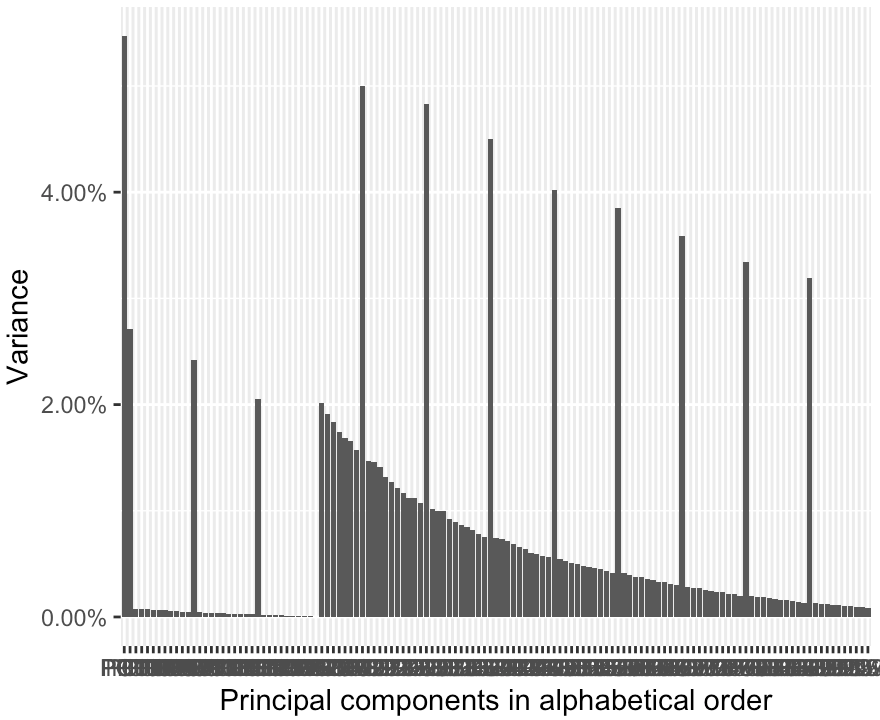
\includegraphics[scale=0.6]{Images/subjectdata_screeplot.png}
			\caption{PCA scree plot (see \ref{incgraphstatspcascreeplot} for component order)}
			\label{subjectdatapcascreeplot}
		\end{figure}
	
		The first principal component covered only 5.47$\%$ of the variance in the subject data, and the first 10 components cumulatively do not cover 50$\%$ of the variance. In addition, the first 2 principal components do not have significantly greater variance than the remainder of the components; this means the biplot visualization is not a good representation of the subject data. T-distributed stochastic neighbor embedding and multidimensional scaling were also conducted on the subject data, but were similarly unreliable.
		
		PCA was also conducted on the INCgraphstats and DECgraphstats datasets. The biplots with labeled vectors and the scree plots are given below.
		
		\begin{figure}[H]
			\centering
			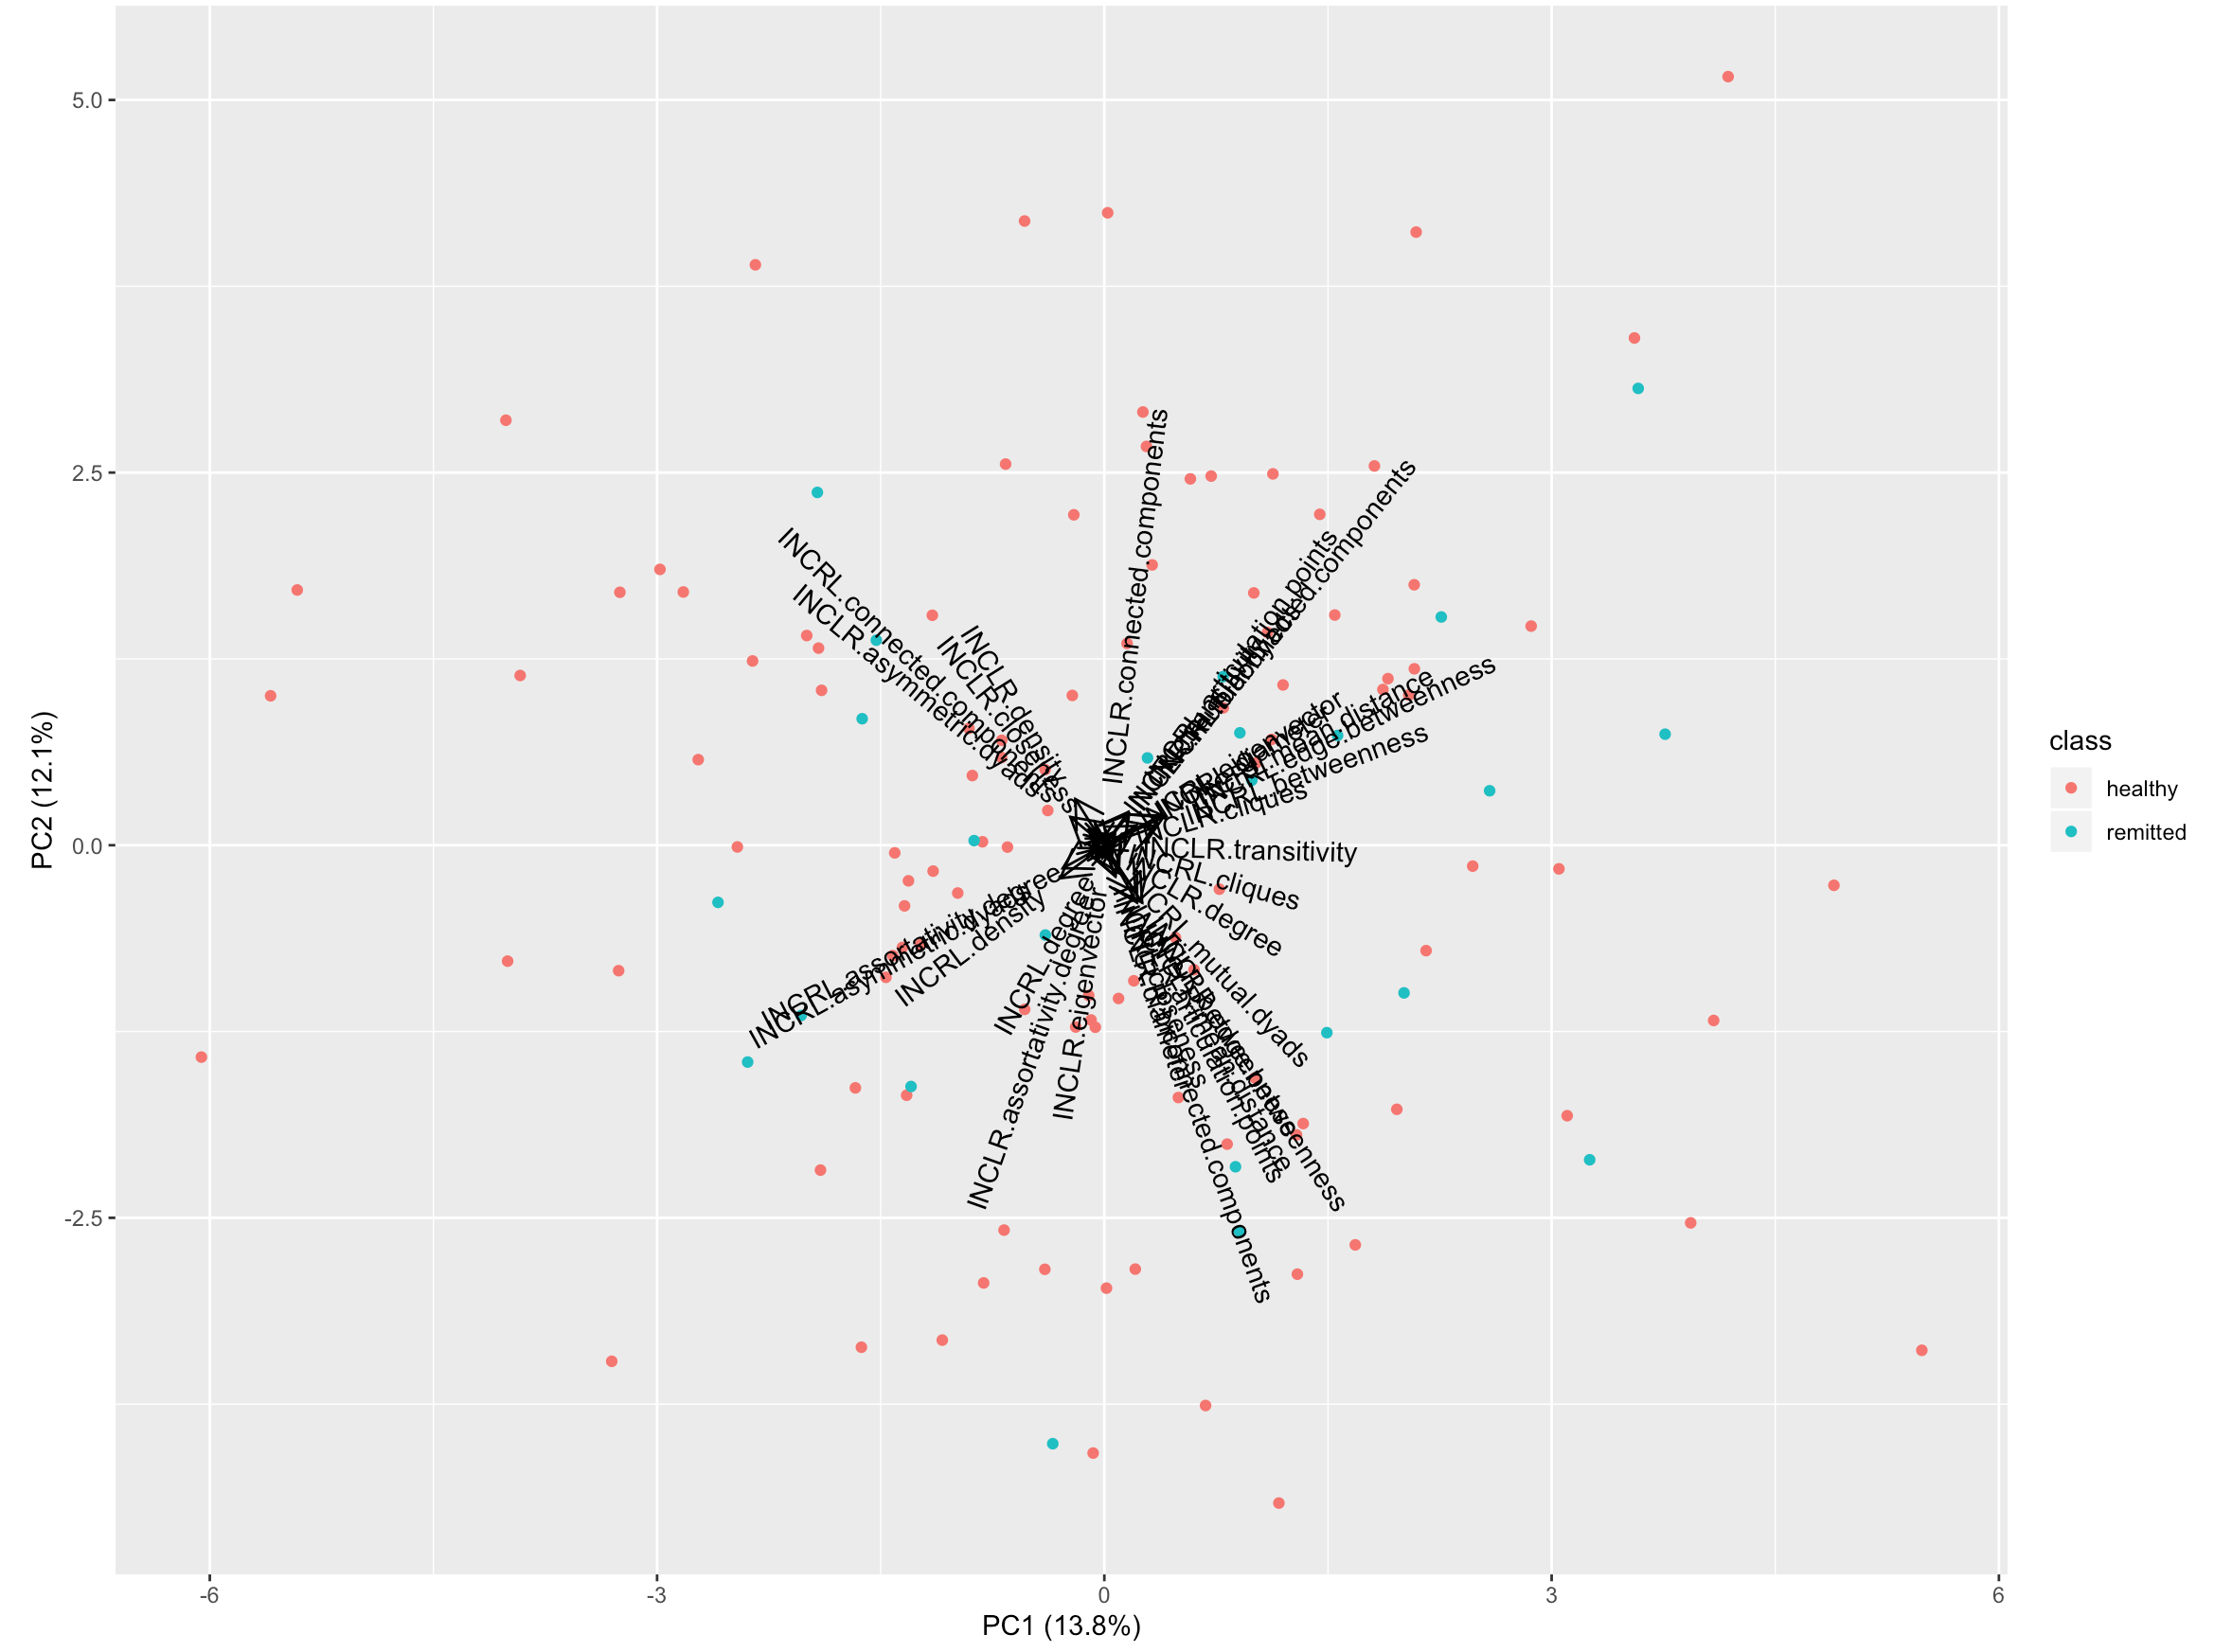
\includegraphics[scale=0.25]{Images/INCgraphstats_biplot.png}
			\caption{Increased emotional response general network characteristics PCA biplot}
			\label{incgraphstatspcabiplot}
		\end{figure}
	
		\begin{figure}[H]
			\centering
			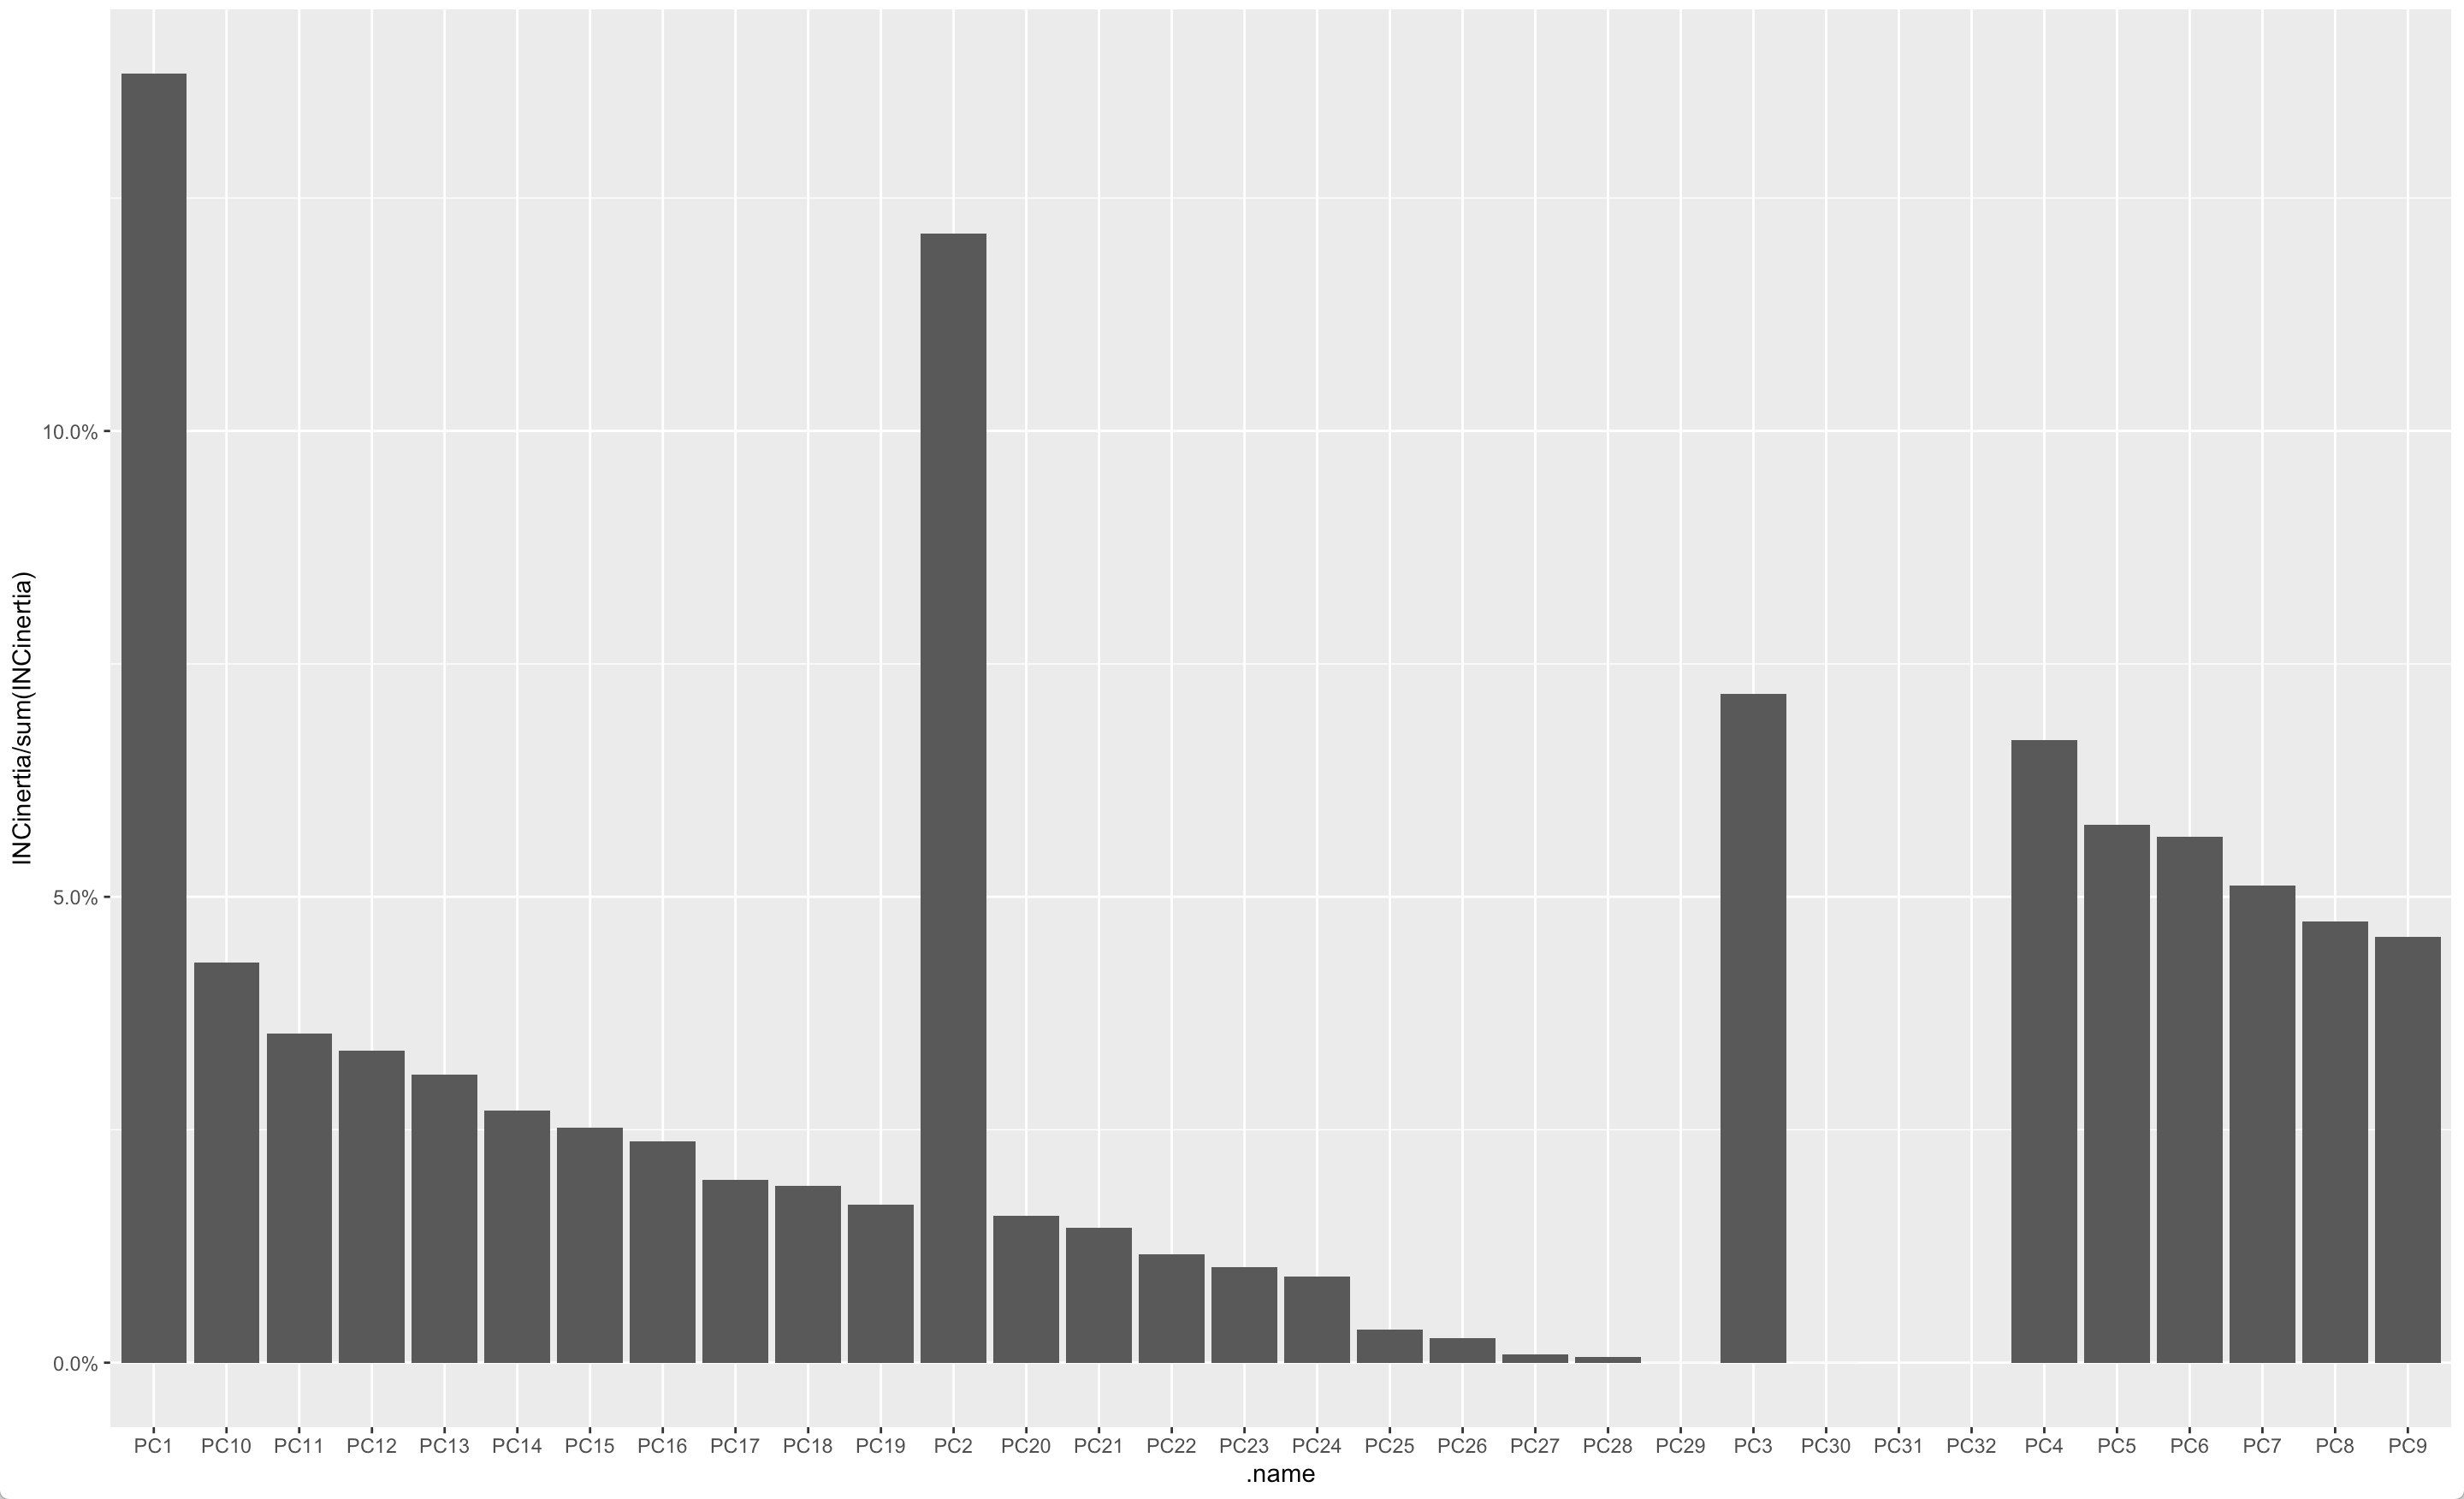
\includegraphics[scale=0.2]{Images/INCgraphstats_screeplot.png}
			\caption{Increased emotional response general network characteristics PCA scree plot}
			\label{incgraphstatspcascreeplot}
		\end{figure}
	
		\begin{figure}[H]
			\centering
			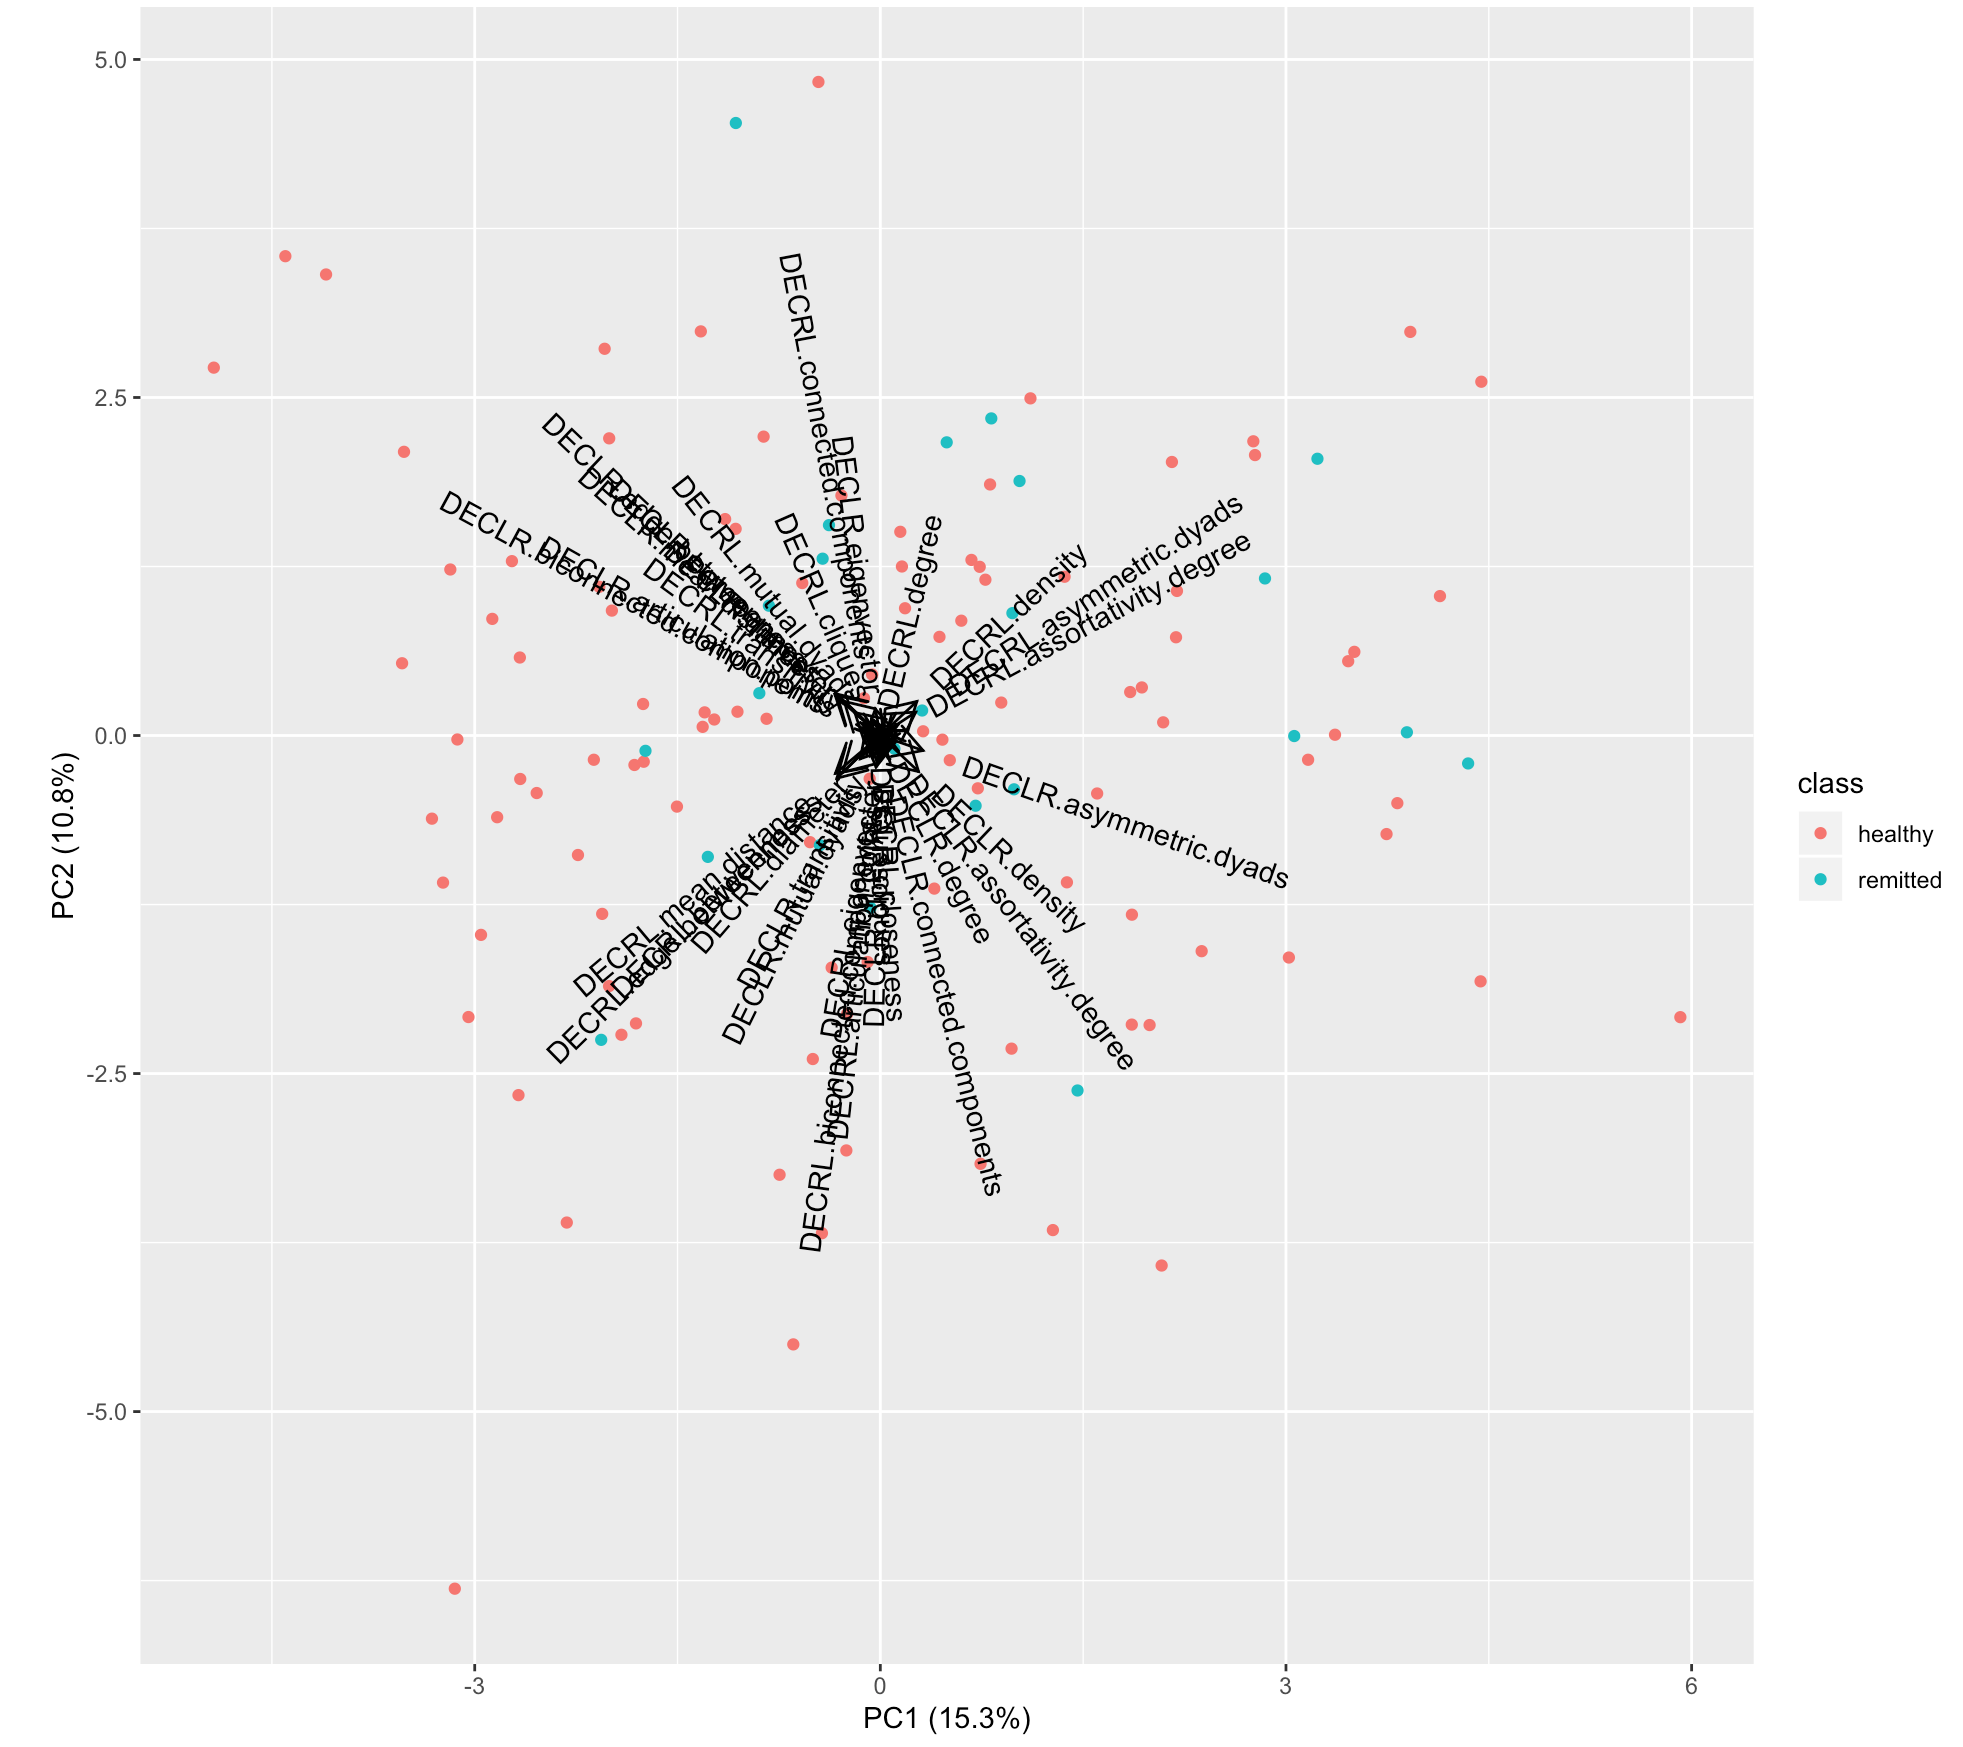
\includegraphics[scale=0.25]{Images/DECgraphstats_biplot.png}
			\caption{Decreased emotional response general network characteristics PCA biplot}
			\label{decgraphstatspcabiplot}
		\end{figure}
		
		\begin{figure}[H]
			\centering
			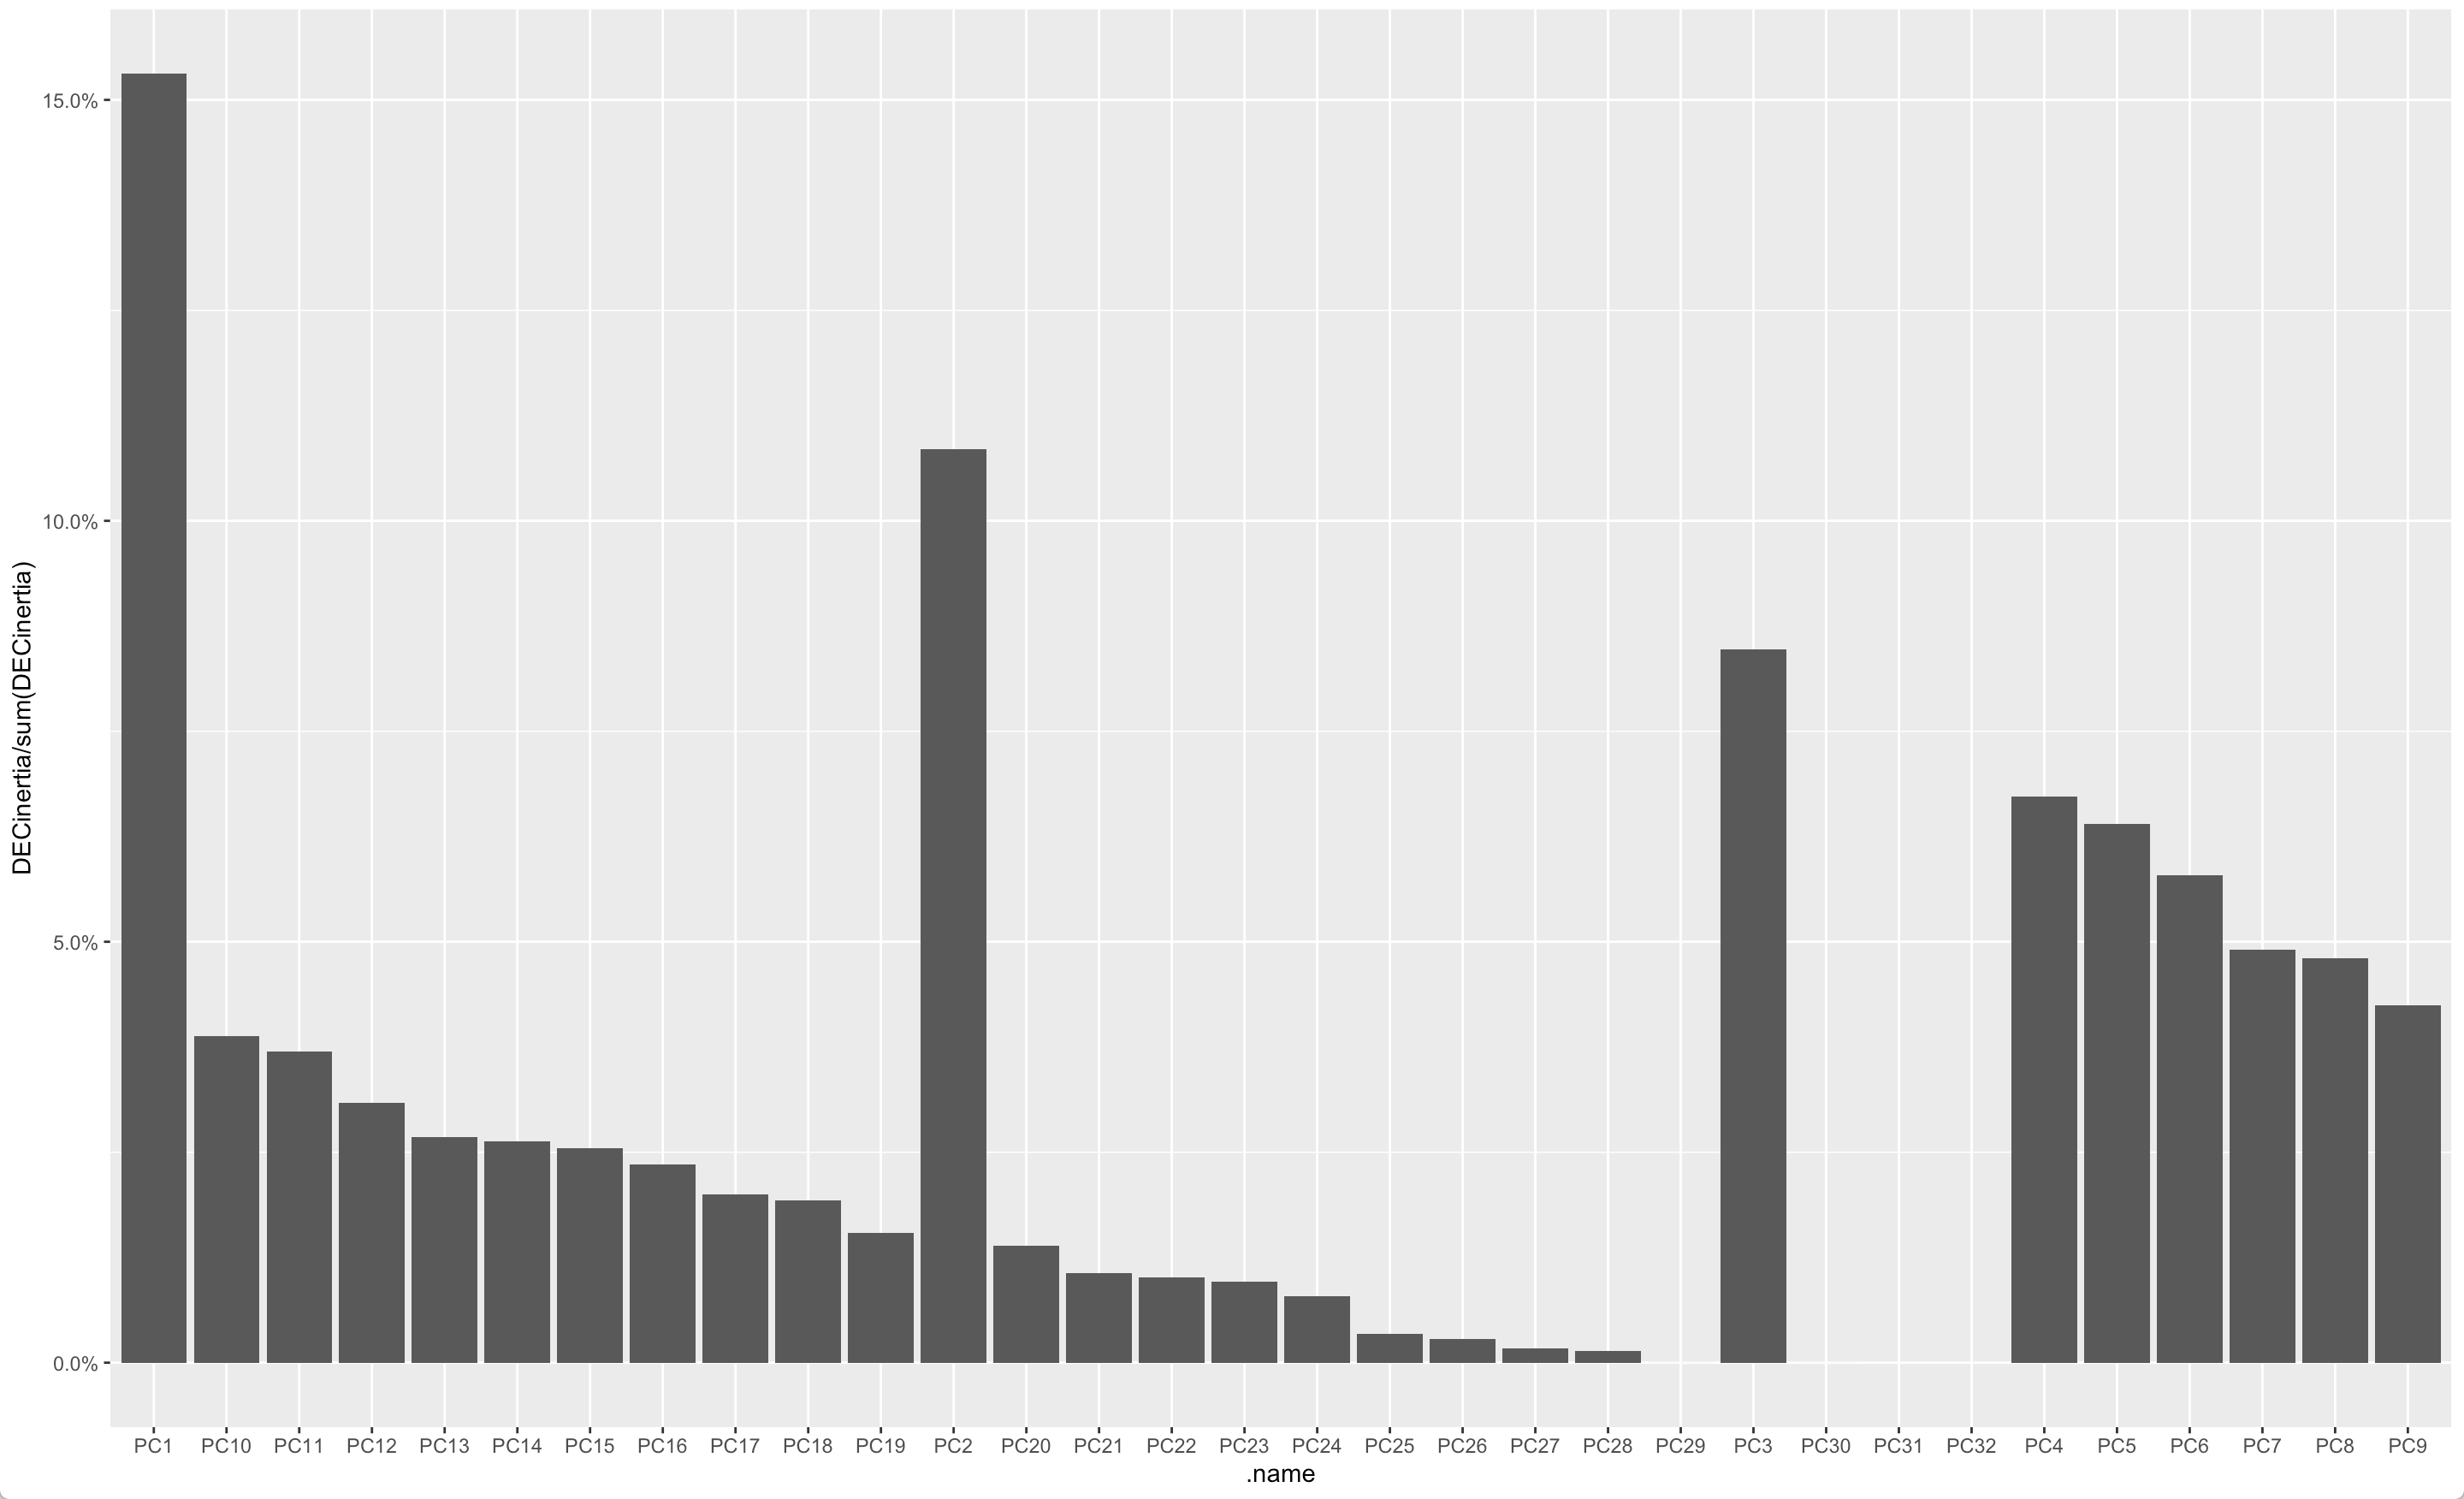
\includegraphics[scale=0.2]{Images/DECgraphstats_screeplot.png}
			\caption{Decreased emotional response general network characteristics PCA scree plot}
			\label{decgraphstatspcascreeplot}
		\end{figure}
		
		The first two principal components cumulatively captured over 20$\%$ of the variance in both the increased and decreased emotional response data, as shown in \ref{incgraphstatspcascreeplot} and \ref{decgraphstatspcascreeplot} respectively. This is still not enough to consider the biplots to be good representations of the data; conclusions should not be drawn from a biplot unless the first 2 components (if the plot is 2 dimensional) account for at least 50$\%$ of the variance in the data. At any rate, neither biplot (\ref{incgraphstatspcabiplot} for increased emotional response and \ref{decgraphstatspcabiplot} for decreased emotional response) shows any clustering.
		
		\section{Machine Learning}
			\subsection{Hierarchical clustering}
			Hierarchical clustering is an unsupervised machine learning technique where each point is initially assigned to its own cluster. The algorithm then iteratively clusters the two clusters who are the closest to eachother; this hierarchical clustering can be traced with a dendrogram \cite{james2013introduction}. The dengrogram for the hierarchical clustering conducted on the subject data using the hclust() function in R is given in \ref{subjectdatadendrogram}.
			
			\begin{figure}[H]
				\centering
				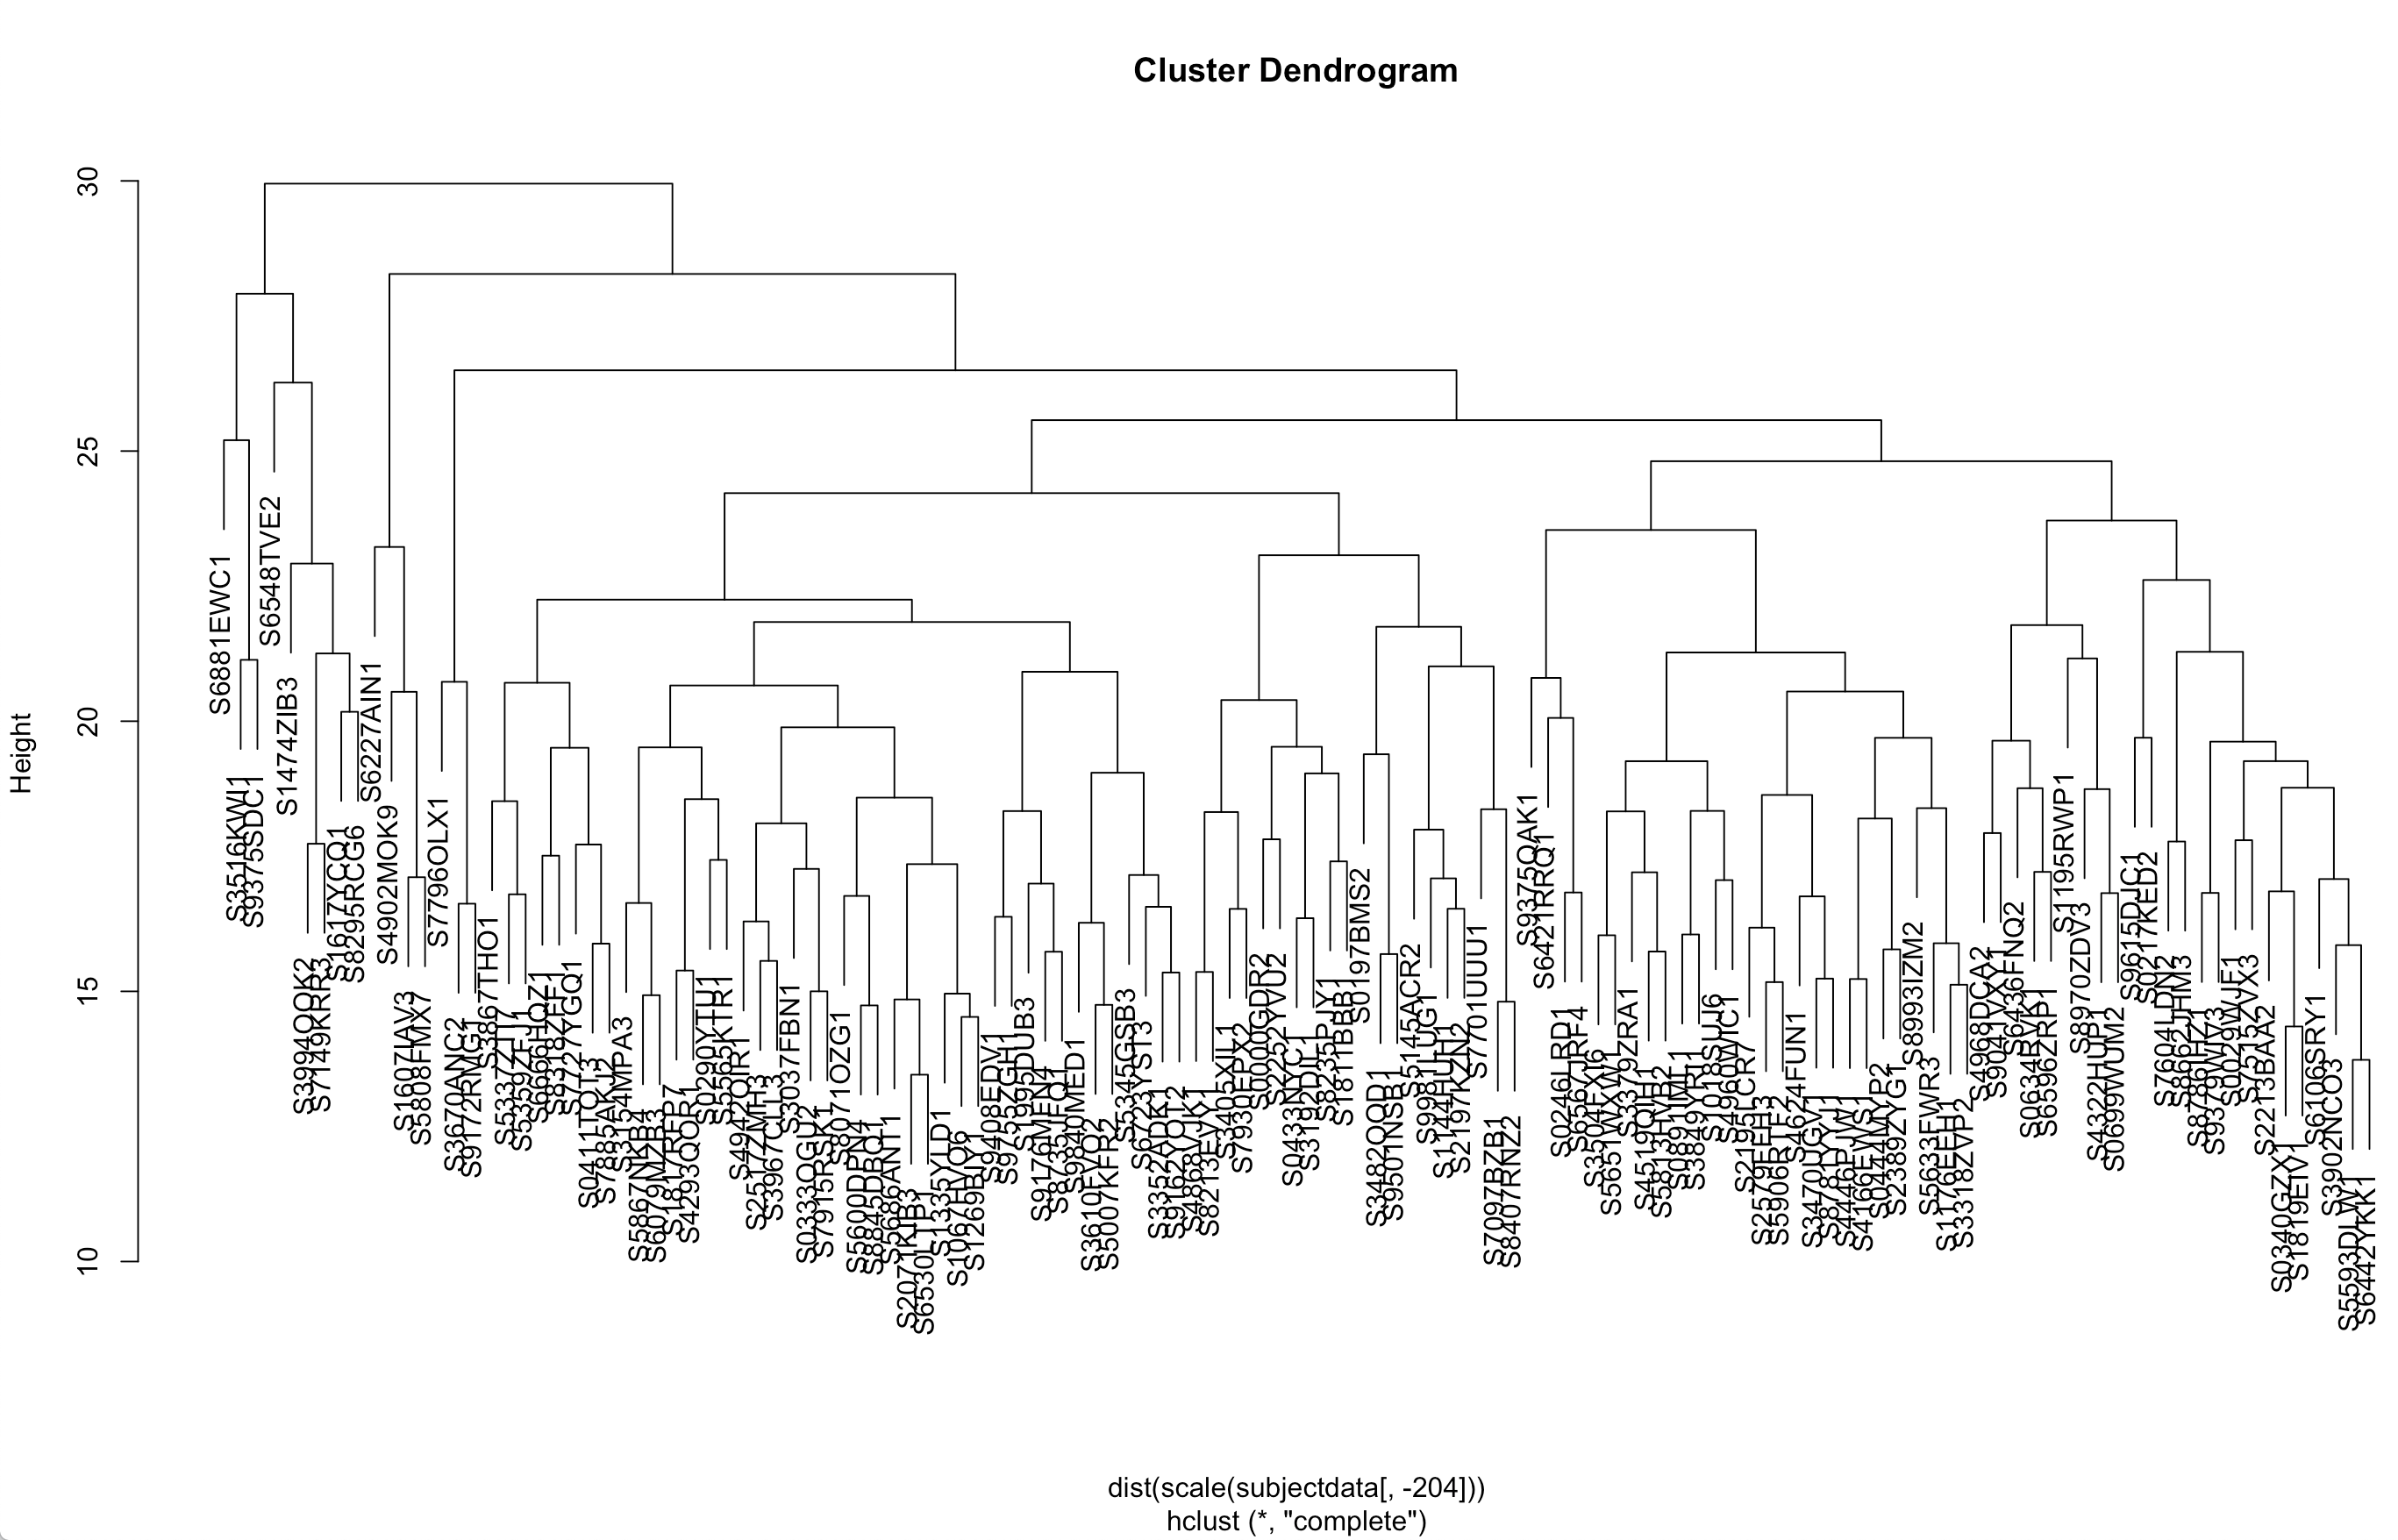
\includegraphics[scale=0.25]{Images/subjectdata_dendrogram.png}
				\caption{Dendrogram}
				\label{subjectdatadendrogram}
			\end{figure}
			
			\begin{figure}[H]
				\centering
				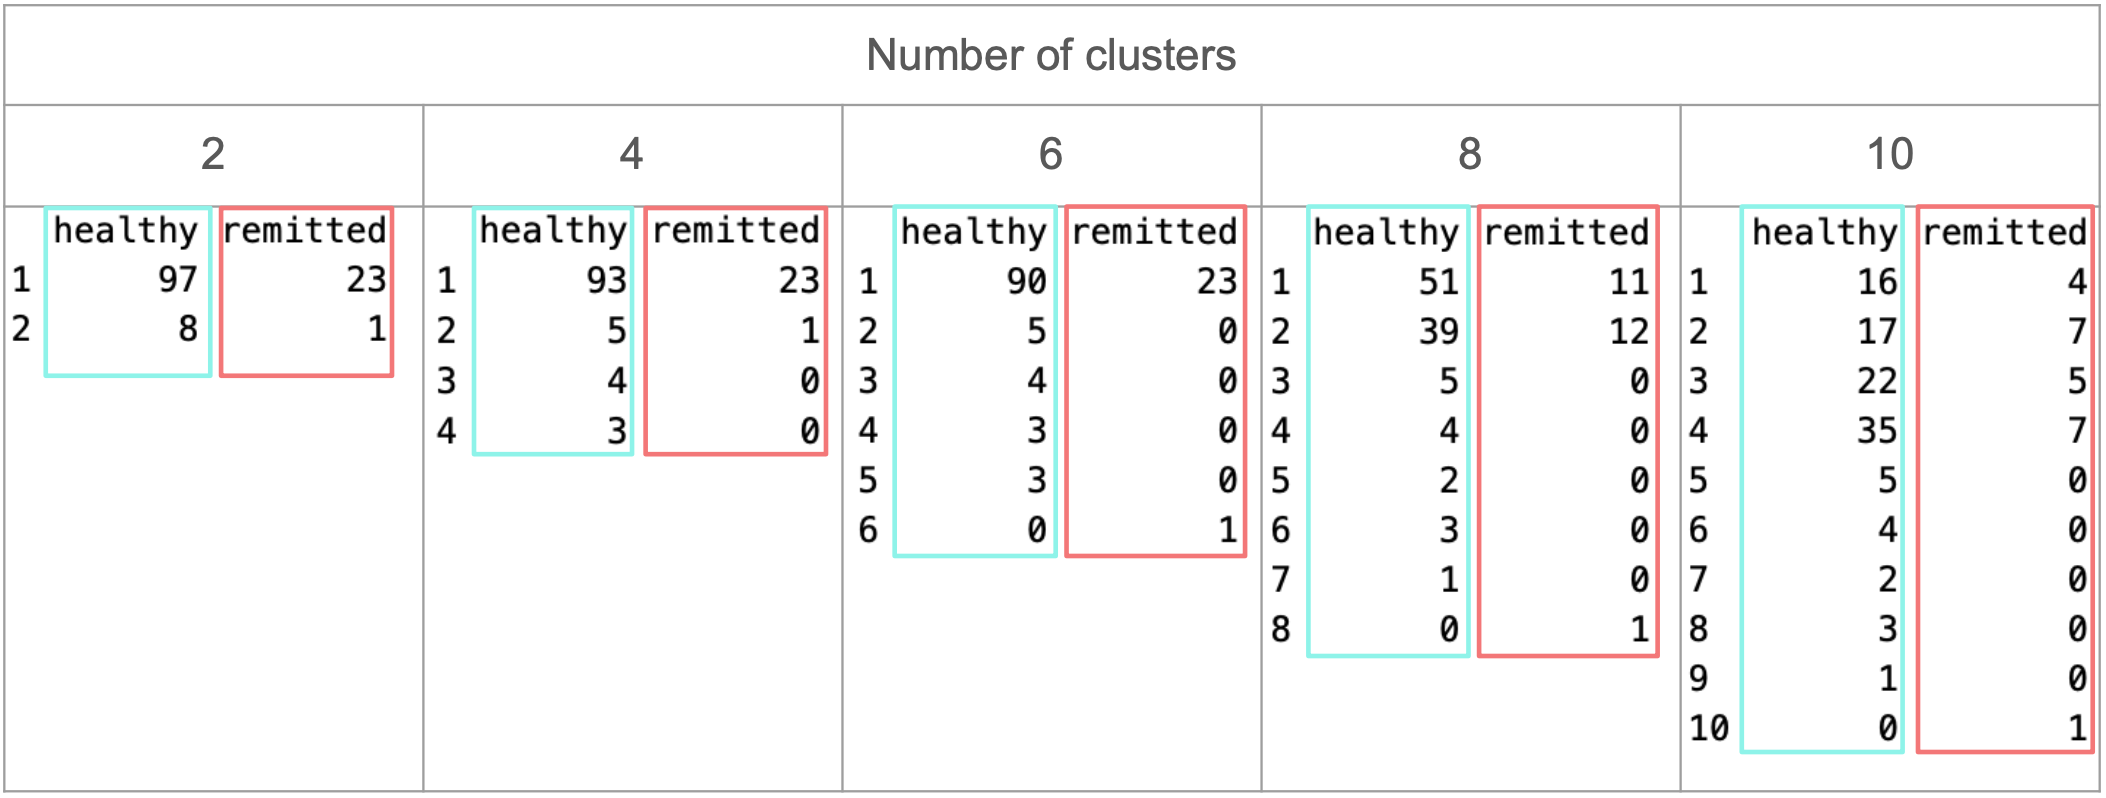
\includegraphics[scale=0.35]{Images/subjectdata_hclust.png}
				\caption{Hierarchical clustering}
				\label{subjectdatahclust}
			\end{figure}
			
			The composition of each cluster can be visualized in a table; see the script subject$\_$data$\_$analysis.R. The results of various clusterings of the subject data is given in \ref{subjectdatahclust}. No matter how many clusters the subject data is broken into, hierarchical clustering never produces a large cluster composed predominantly of one class or another. For example, consider cluster 1 in the columns for 2, 4, and 6 clusters; it contains 113 of the 129 subjects. The fact that the majority of the subjects here are healthy is merely a reflection of the makeup of the subject population. When this large cluster is split up (into clusters 1 and 2 in the column for 8 clusters), the remitted subjects are split evenly into the two resultant clusters. This indicates that the differences that the clustering is identifying do not divide healthy subjects from remitted. It may be useful to run a separate analysis on the subjects in certain clusters to determine what is causing them to be grouped together; the commands that produce lists of subject identifiers by cluster are in the script subject$\_$data$\_$analysis.R.

			\subsection{k-means}
			K-means is another unsupervised machine learning technique. The user specifies a number of clusters $k$ and the algorithm initially chooses k centroids. Initial clusters are determined by assigning each point to the nearest centroid, in of Euclidean distance. Each centroid is then shifted to the mean of its cluster, after which the points are reassigned to new clusters. The algorithm repeats this process until there is no change in the clusters between runs or until some previously defined stopping condition is met \cite{james2013introduction}. The kmeans() function was used in R.
			
			Like with hierarchical clustering, the composition of each k-means cluster can be visualized in a table; see the script subject$\_$data$\_$analysis.R. The results of the k-means clustering display the same trends found in the hierarchical clustering: as $k$ increases, the remitted subjects are split evenly between the largest clusters.
						
			\subsection{k-nearest neighbors}
			K-nearest neighbors (KNN) is a supervised machine learning technique that classifies test cases according to their proximity to training cases. The user specifies the number of nearest neighbors $k$ to consider, and the algorithm classifies each test case as the class of the majority of the $k$ closest training cases \cite{james2013introduction}.
			
			Scripts were written to measure the accuracy of the KNN models by calculating their precision and recall,\\ where $ \text{precision} = \dfrac{\text{true positives}}{\text{true positives}+\text{false positives}} $ \\ and $ \text{recall} = \dfrac{\text{true positives}}{\text{true positives}+\text{false negatives}} $. \\ These values were calculated for each $k$, after which precision-recall curves were plotted; see the scripts knn$\_$binary$\_$loop.R and precision$\_$recall$\_$curves.R. The precision-recall curve for the KNN models built from the subject data is given in \ref{subjectdataprecisionrecall}.
			
			\begin{figure}[H]
				\centering
				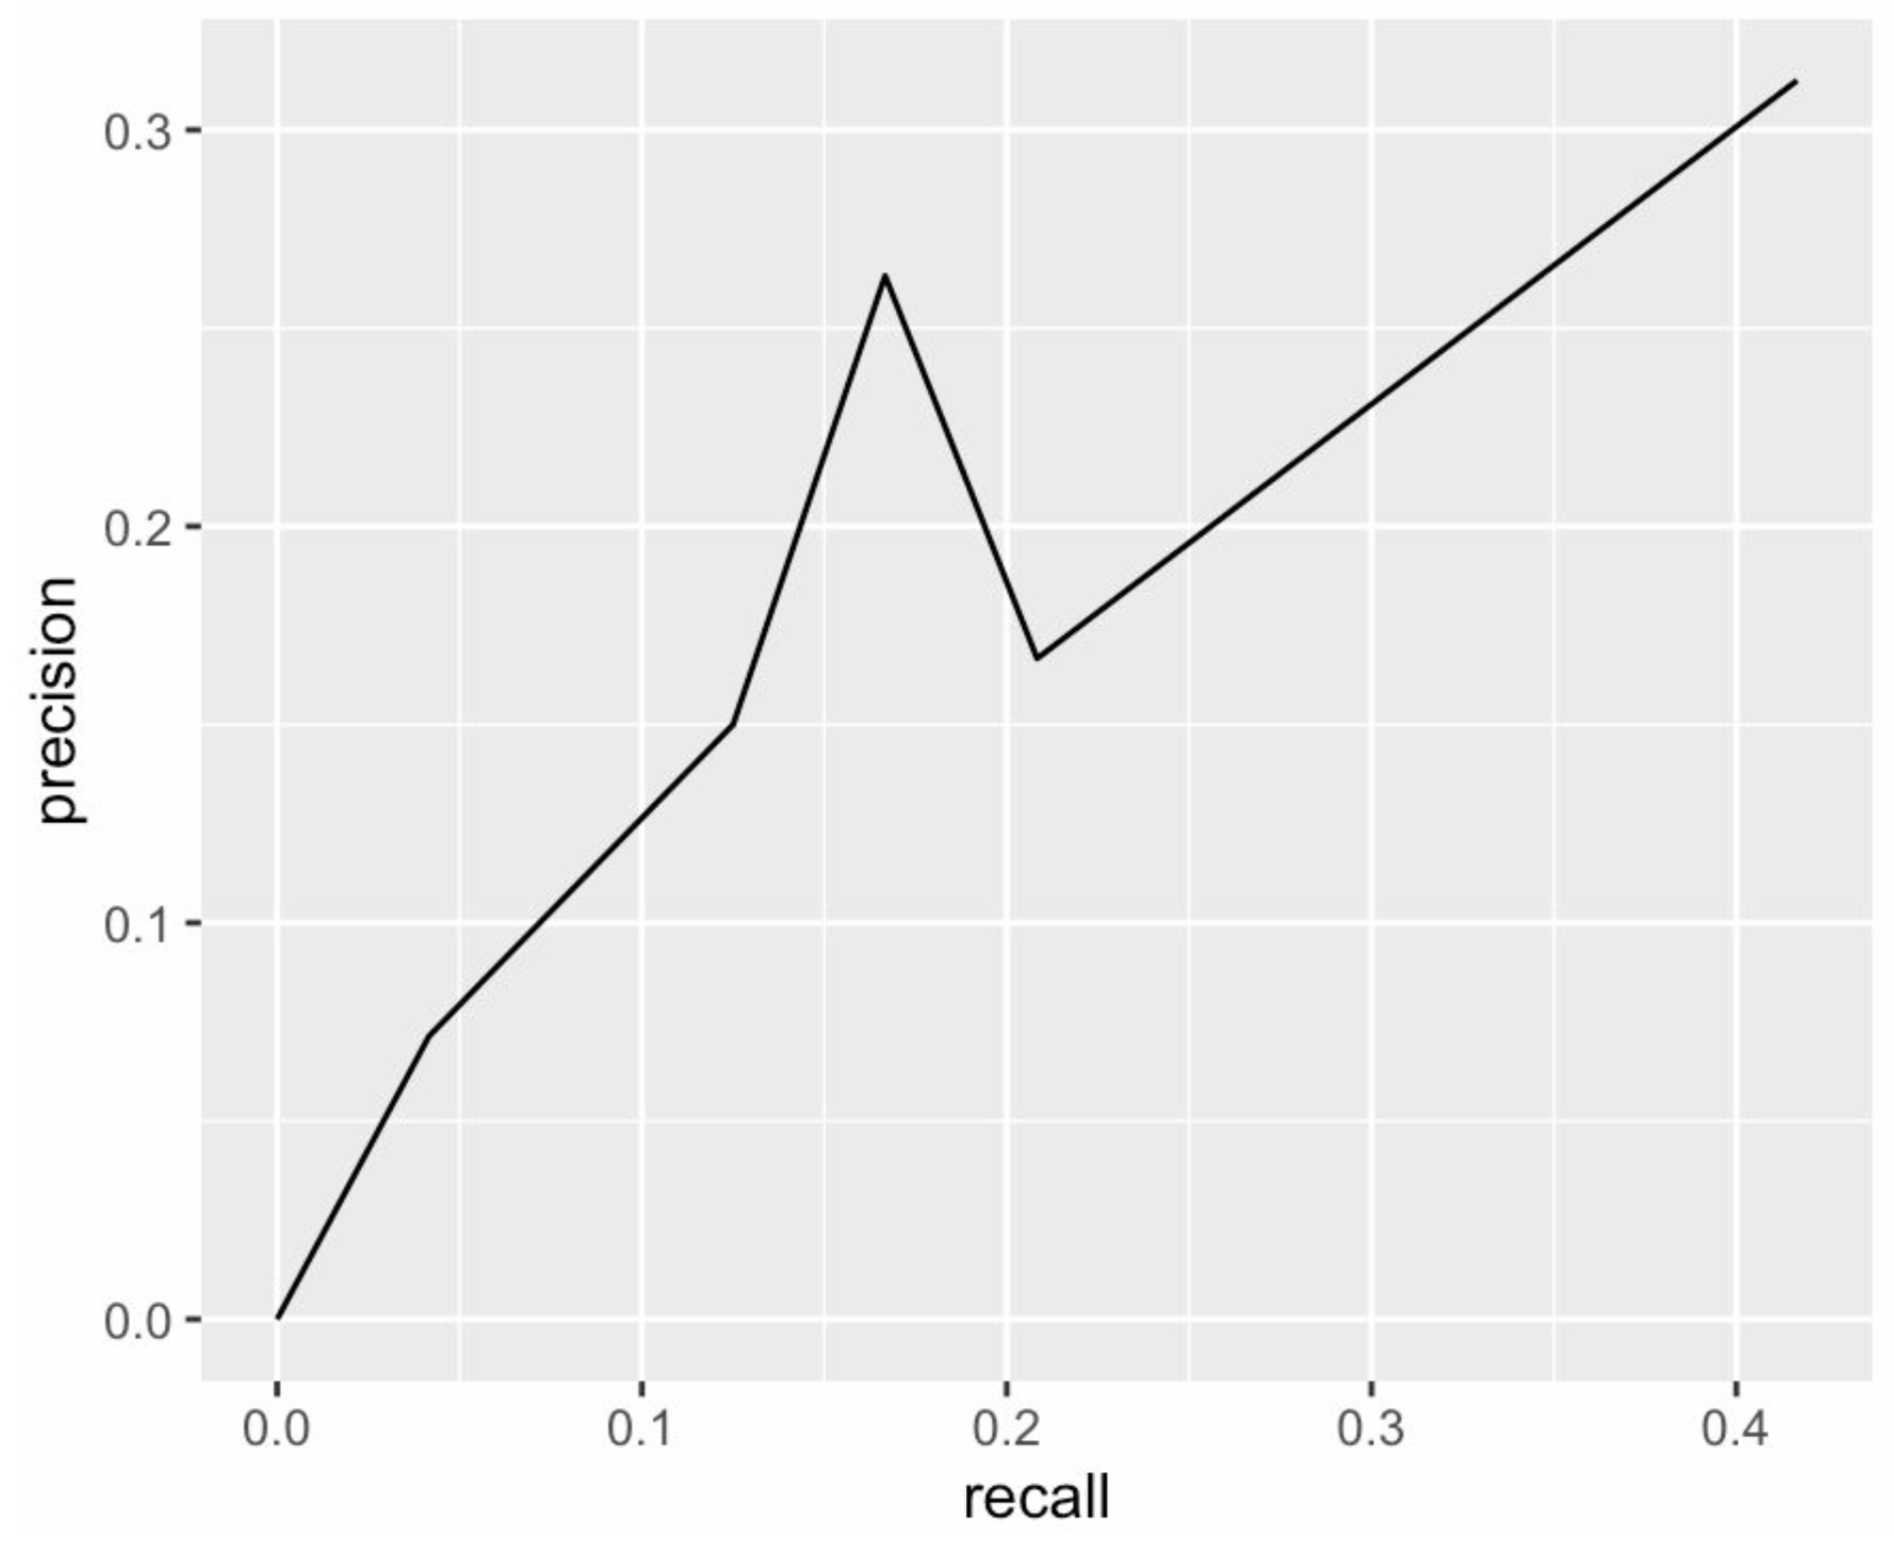
\includegraphics[scale=0.4]{Images/subjectdata_precisionrecall.png}
				\caption{Precision-recall curve}
				\label{subjectdataprecisionrecall}
			\end{figure}
			
			A perfect model would predict with 100$\%$ precision and 100$\%$ recall. However, even the best KNN model only classified with approximately 30$\%$ precision and 40$\%$ recall; it is completely unreliable.
			
		\chapter{Feature Selection}
		Machine learning techniques can be less effective on high dimensional datasets that have many irrelevant features. To attempt to reduce the noise in the subject data, feature selection was performed using the scikit-learn package in Python. A logistic model was used with recursive feature elminination, a wrapper function. It iteratively builds predictive models, ranks subsets of features based on model accuracy, and then removes the features with the lowest contributions from the existing set \cite{paul_2018}.
		
		Three new datasets were constructed, one containing 80$\%$ of the total features, one containing 50$\%$, and one containing 30$\%$; see the script feature$\_$selection.py. The analysis described in the Dimensionality Reduction and Machine Learning chapter was repeated on each of these datasets in R after running the script import$\_$selected$\_$features.R. For example, the biplot and scree plot for the PCA conducted on the 30$\%$ dataset are given in figures \ref{rfe60biplot} and \ref{rfe60screeplot} respectively.
		
		\begin{figure}[H]
			\centering
			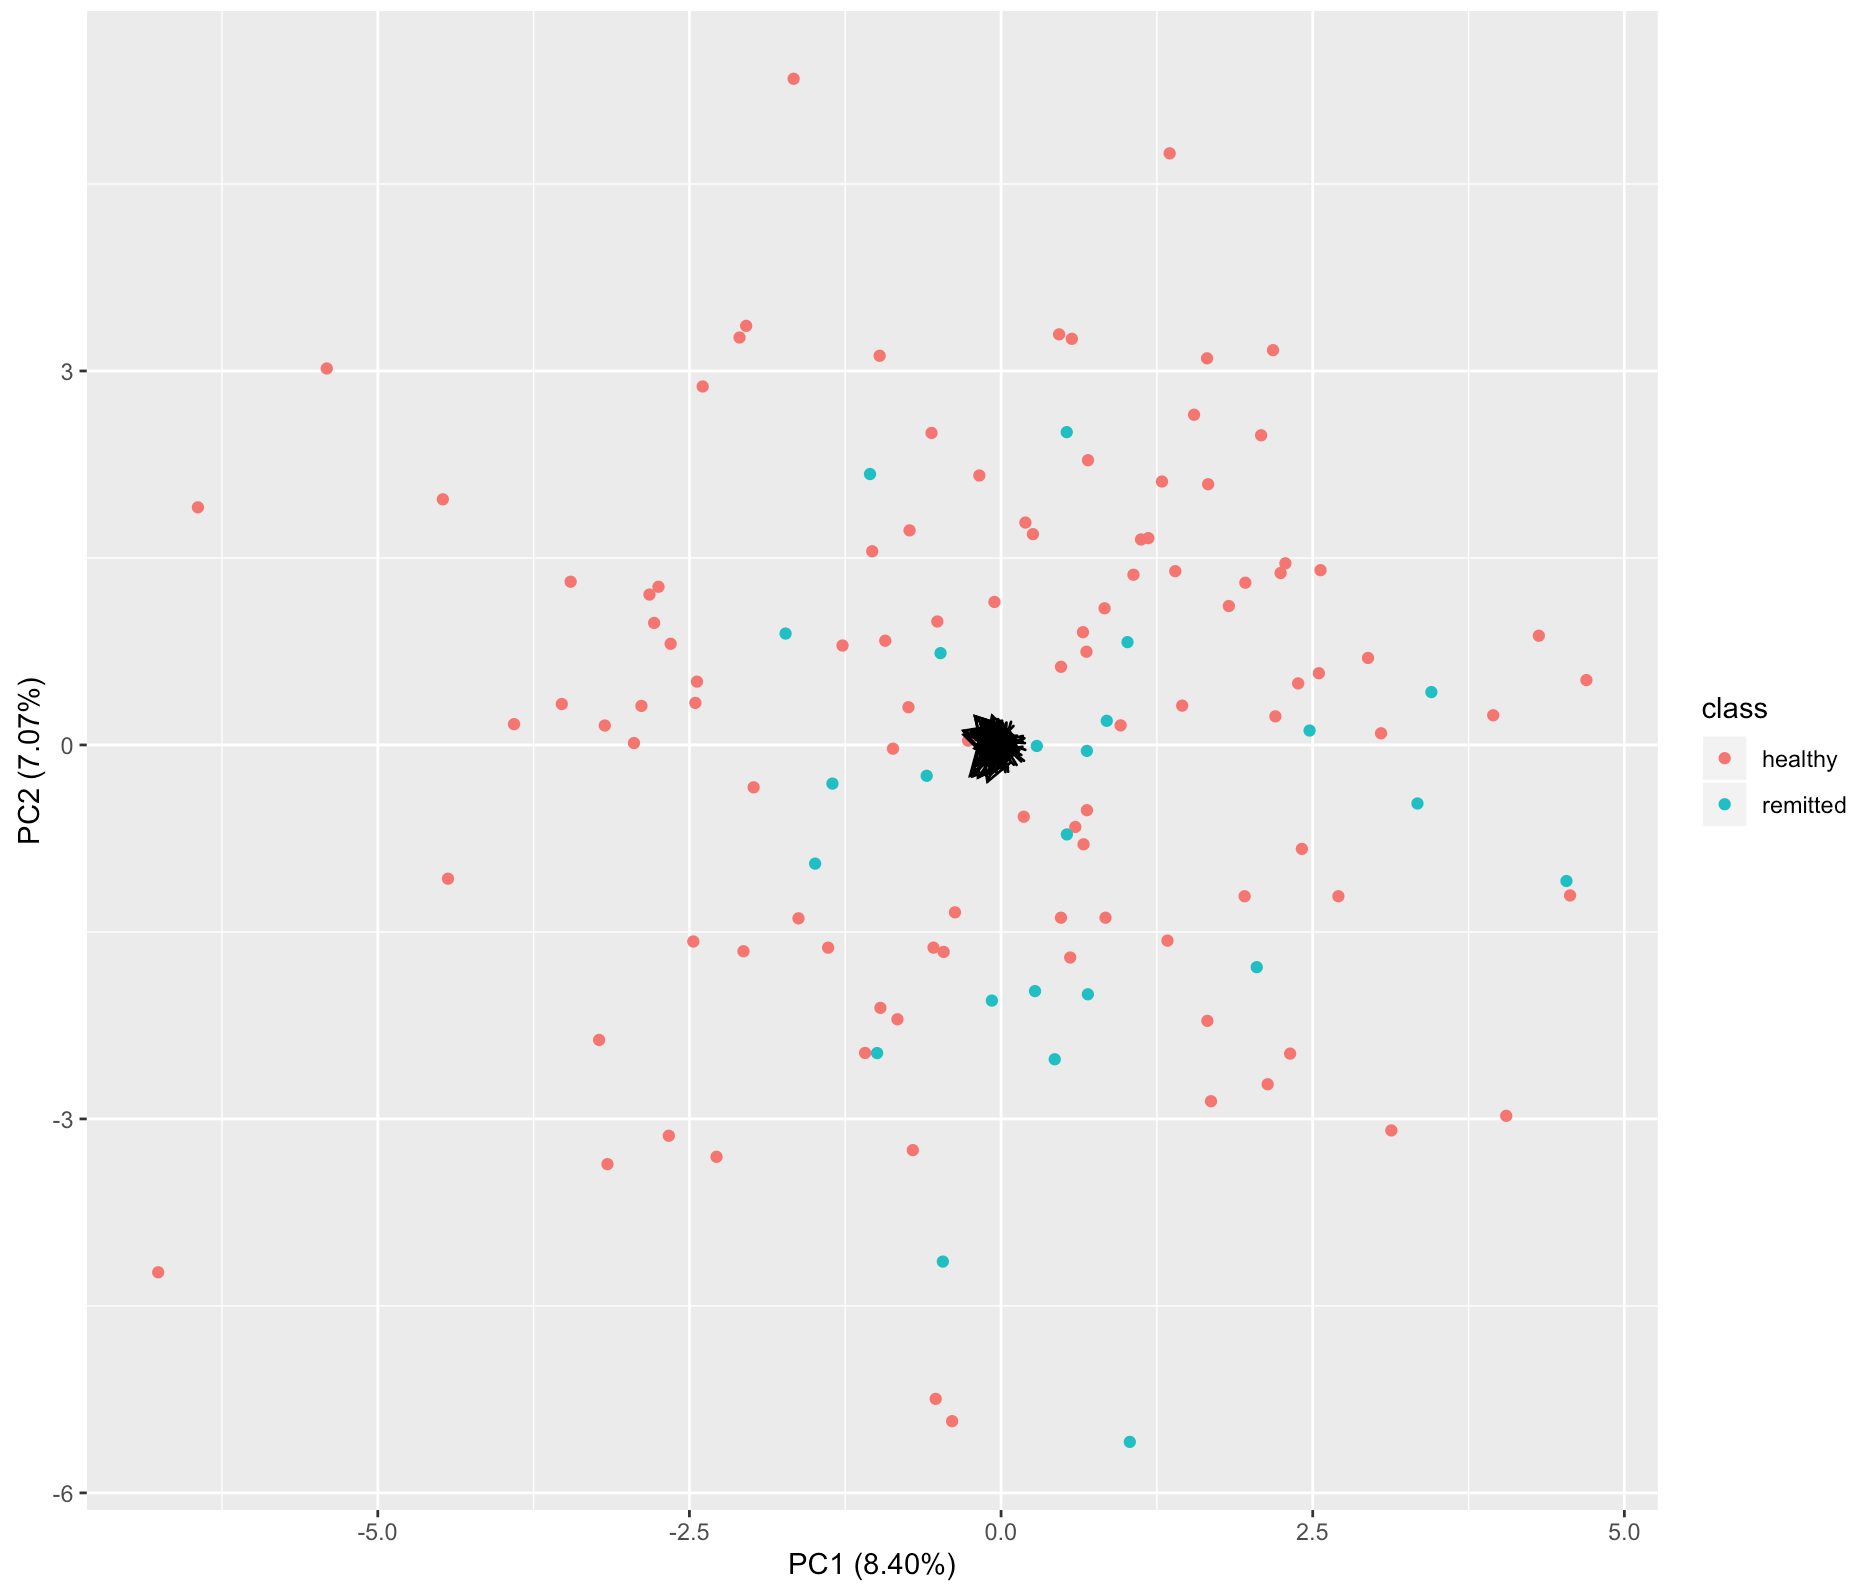
\includegraphics[scale=0.2]{Images/rfe60_biplot.png}
			\caption{30$\%$ dataset PCA biplot}
			\label{rfe60biplot}
		\end{figure}
	
		\begin{figure}[H]
			\centering
			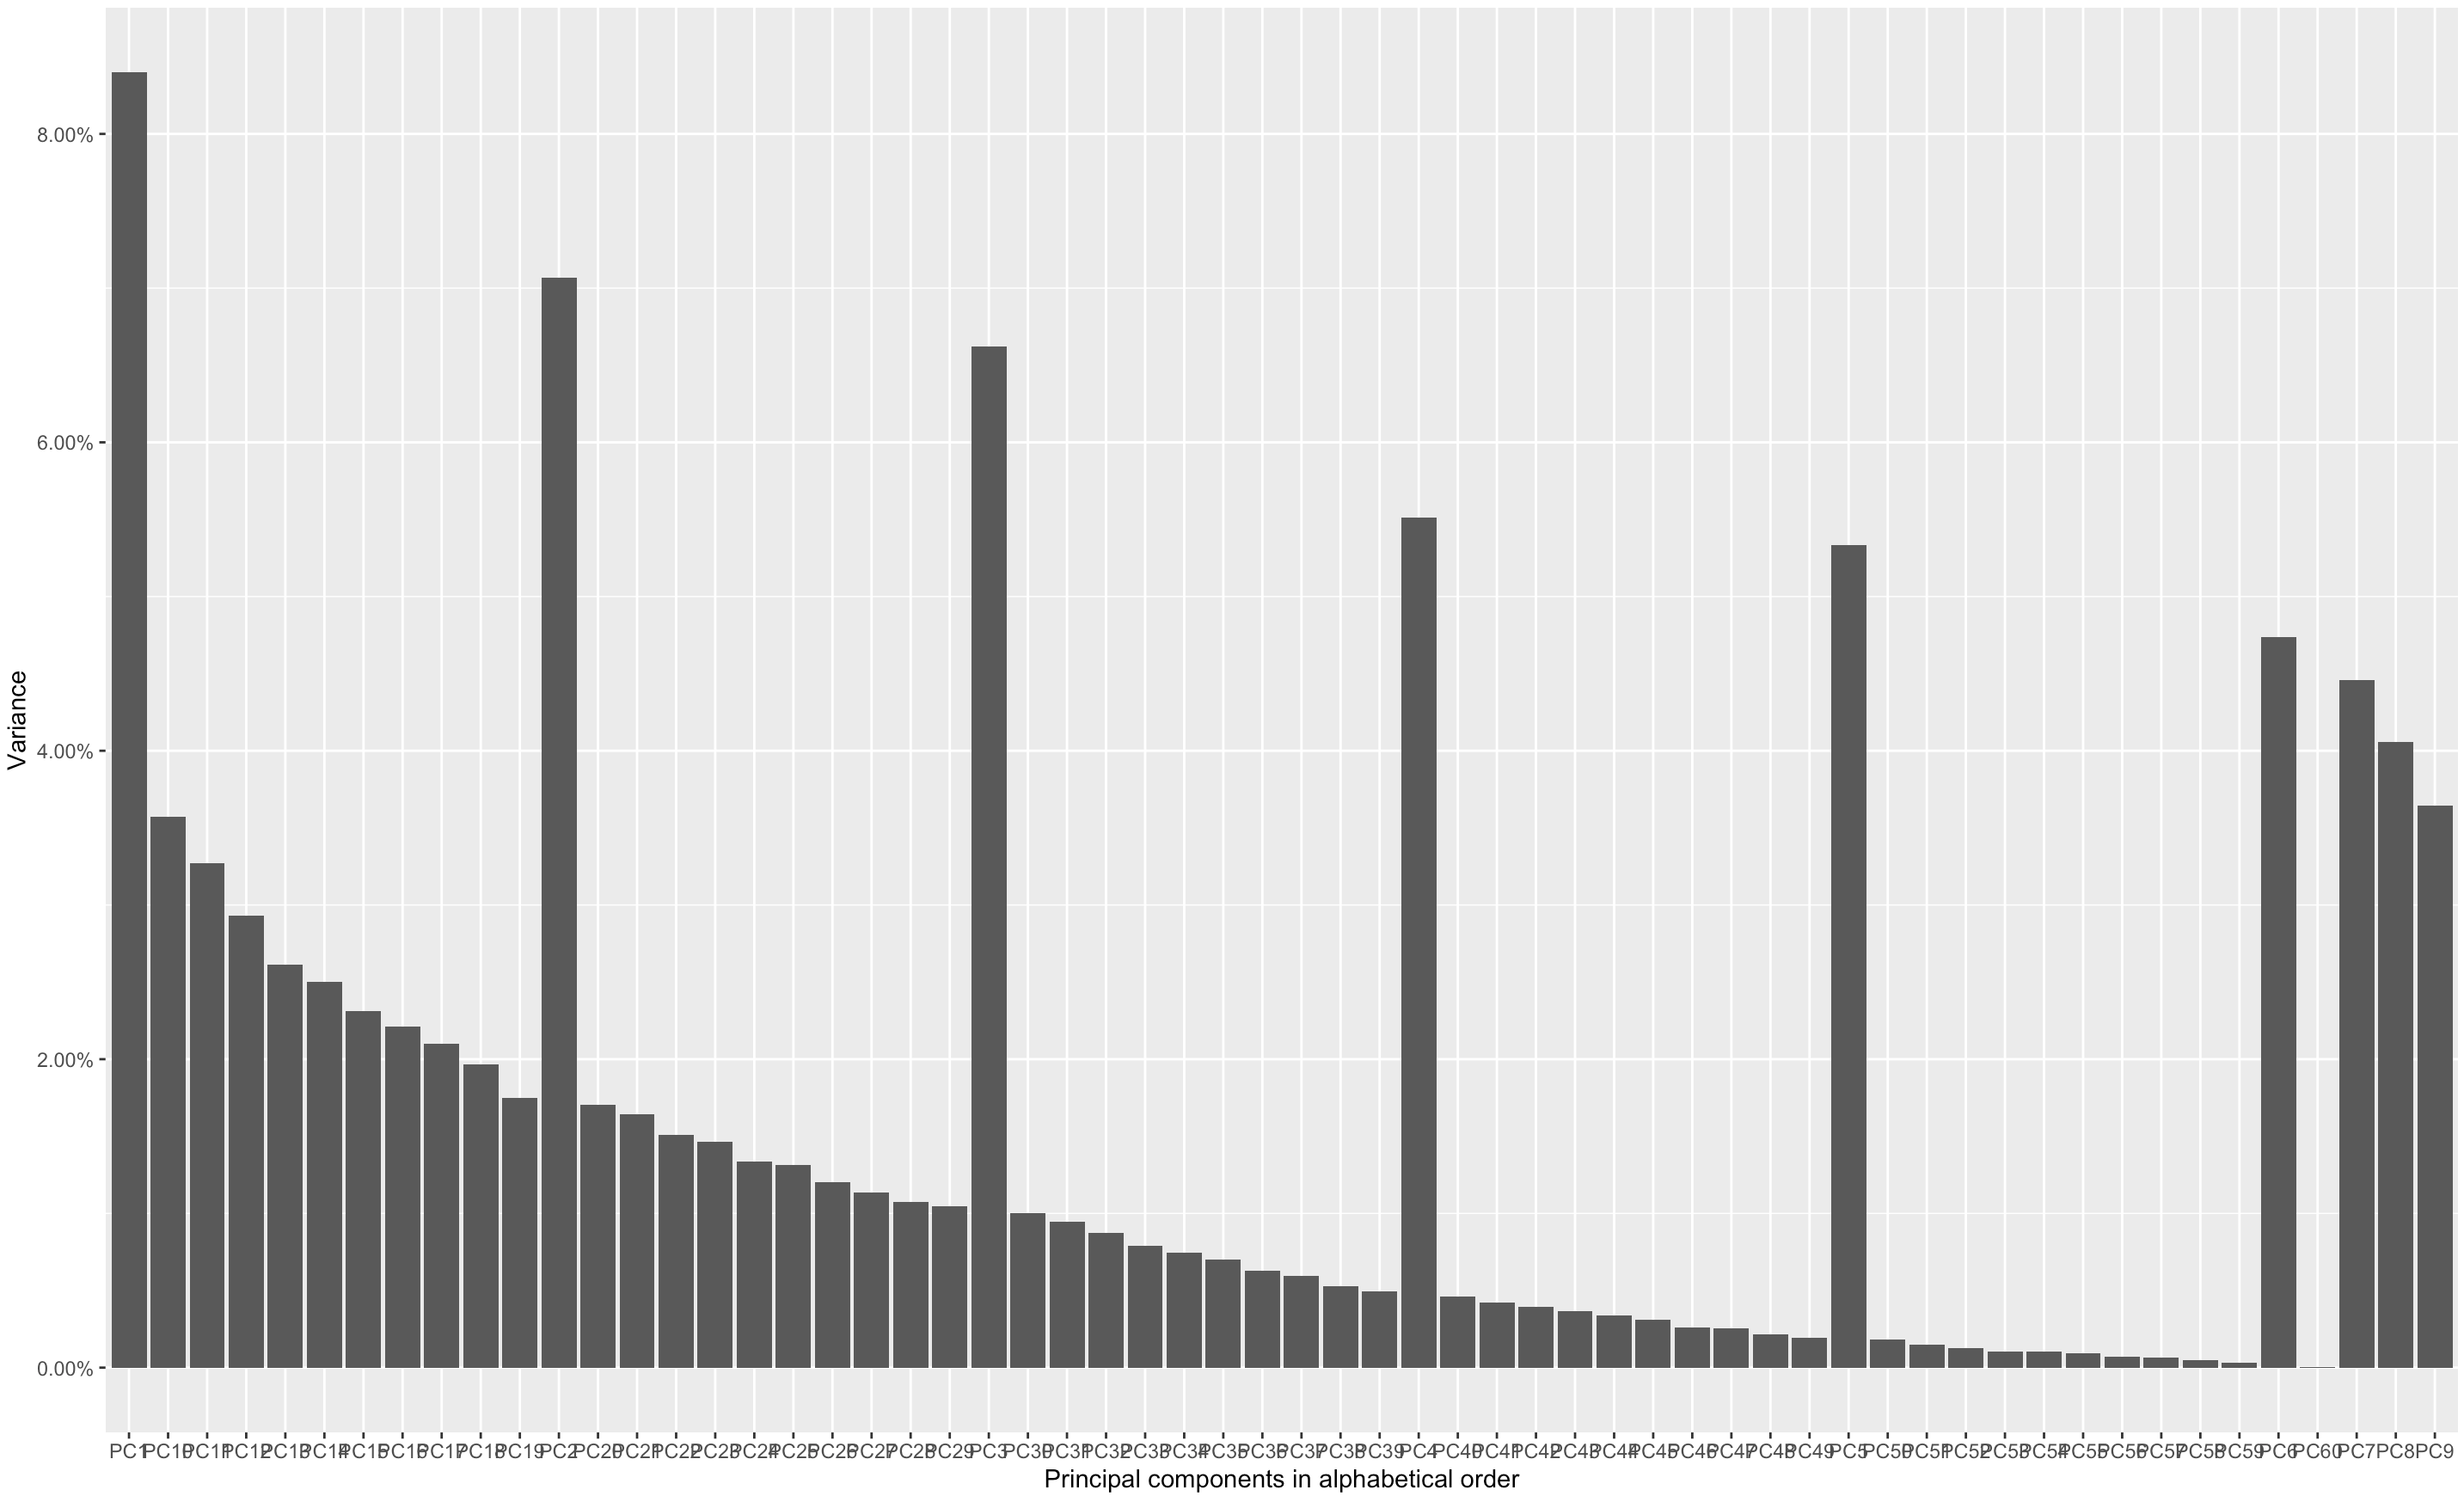
\includegraphics[scale=0.2]{Images/rfe60_screeplot.png}
			\caption{30$\%$ dataset PCA scree plot}
			\label{rfe60screeplot}
		\end{figure}
		
		This PCA is a bad representation of the data for the same reasons that \ref{subjectdatapcabiplot} is. For example, the first principal component accounts for less than 8.25$\%$ of the variance. This is the case for the PCA conducted on the 50$\%$ dataset and that conducted on the 80$\%$ dataset as well. The trends in the subject data are reflected in the smaller datasets. This also holds true for hierarchical clustering, k-means, and KNN.
		
		\begin{figure}[H]
			\centering
			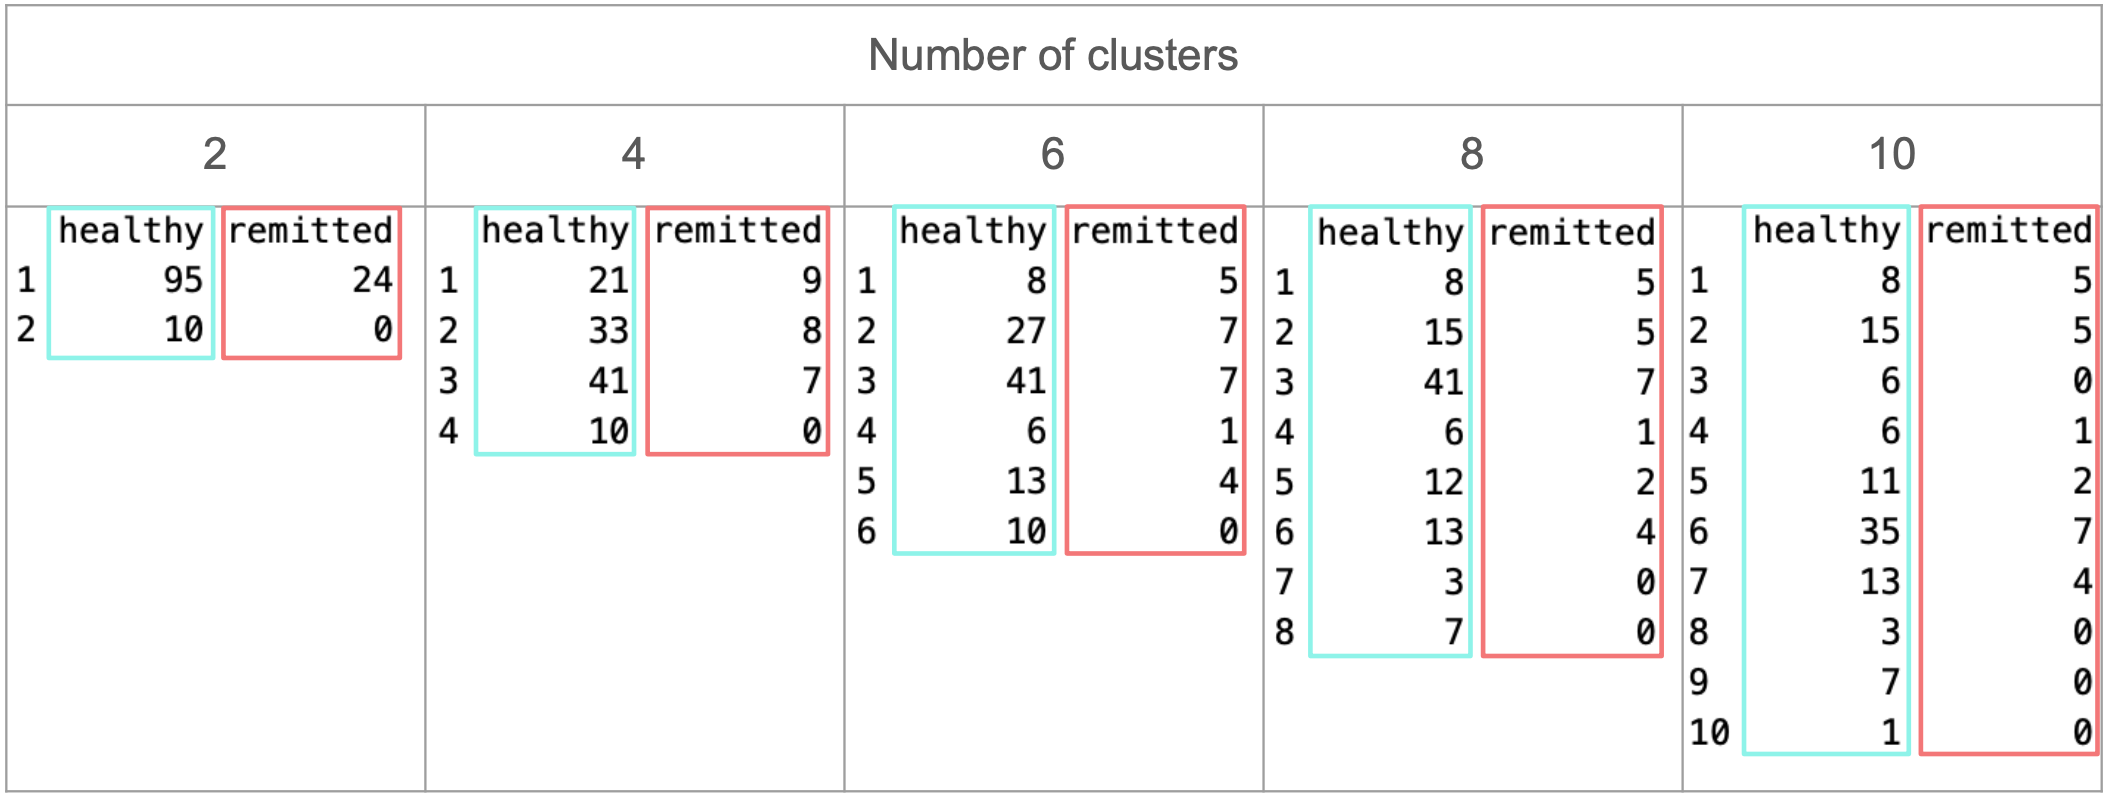
\includegraphics[scale=0.3]{Images/rfe101_hclust.png}
			\caption{50$\%$ dataset hierarchical clustering}
			\label{rfe101hclust}
		\end{figure}
		
		\begin{figure}[H]
			\centering
			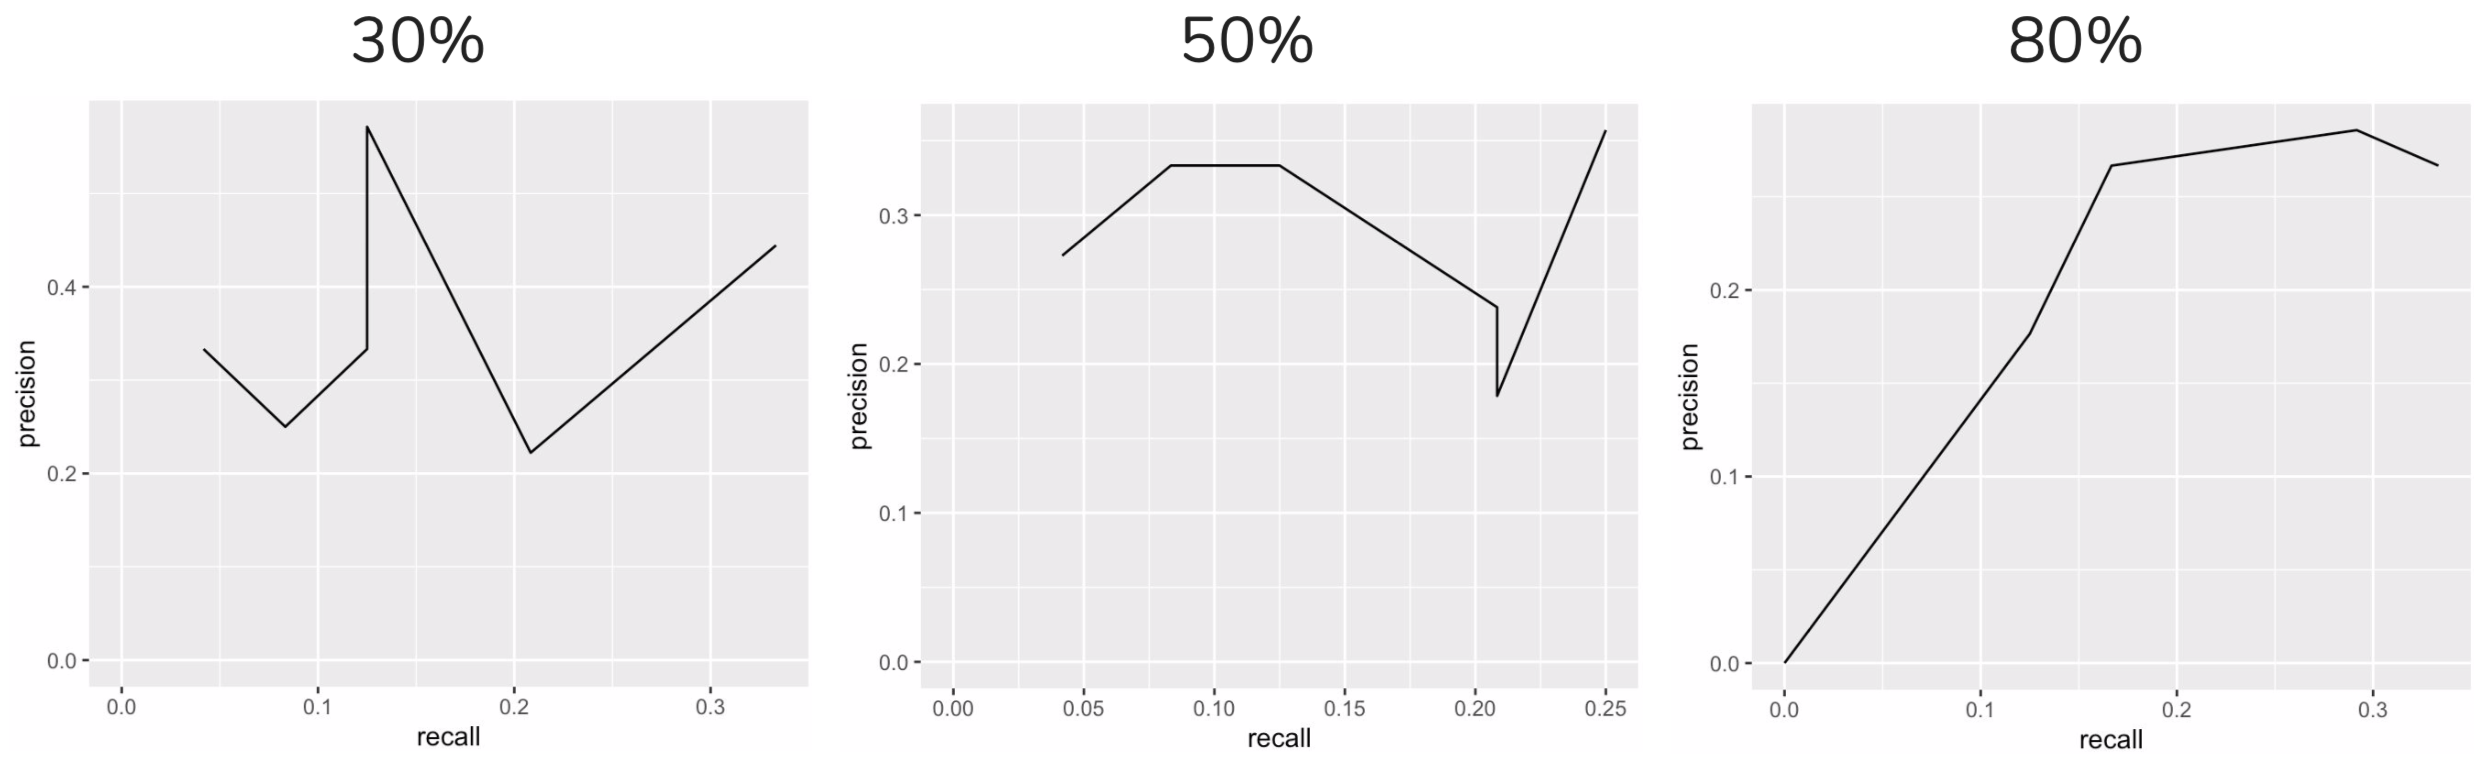
\includegraphics[scale=0.3]{Images/featureselection_precisionrecall.png}
			\caption{Selected feature datasets' precision-recall curves}
			\label{featureselectionprecisionrecall}
		\end{figure}
			
		The hierarchical clustering carried out on the 30$\%$ dataset, displayed in figure \ref{rfe101hclust}, displays the same behavior that the hierarchical clustering on the subject data (figure \ref{subjectdatahclust}) does. Similarly, the precision-recall curves for all three selected feature datasets, displayed in figure \ref{featureselectionprecisionrecall}, show that the KNN models constructed from selected features do not predict with significantly greater accuracy than those constructed from the whole dataset (subject data). For example, one KNN model from the 30$\%$ dataset predicts with greater precision than the best subject data model (over 50$\%$ compared to approximately 30$\%$ for the subject data) but at the cost of greatly reduced recall (less than 15$\%$ compared to approximately 40$\%$ for the subject data). None of the models can be considered accurate predictors.
		
		\chapter{Conclusions and Next Steps}
		The results suggest that network metrics derived from dynamic signatures inferred from fMRI data are not sufficient to consistently classify between healthy and remitted subjects on their own. They also may indicate that connectivity patterns concerning the amygdala-hippocampal complex do not differ significantly between healthy and remitted subjects. However, the remitted patient sample was far smaller than the healthy subject pool, which may have biased the results. Thus, further research would ideally involve a larger number of healthy subjects and subjects who, at the time of data collection, were diagnosed with MDD. It would also include a wider range of machine learning and feature selection techniques, as well as motif searches in the whole networks.
		
\bibliographystyle{plain}
\bibliography{Bibliography}

\end{document}
